% Arquivo LaTeX de exemplo de disserta?o/tese a ser apresentados à CPG do IME-USP
%
% Vers? 5: Sex Mar  9 18:05:40 BRT 2012
%
% Cria?o: Jesus P. Mena-Chalco
% Revisão: Fabio Kon e Paulo Feofiloff
%
% Obs: Leia previamente o texto do arquivo README.txt

\documentclass[11pt,twoside,a4paper]{book}

% ---------------------------------------------------------------------------- %
% Pacotes
\usepackage{fontspec}
\usepackage{polyglossia}
\setdefaultlanguage{brazil}

\usepackage{graphicx}           % usamos arquivos pdf/png como figuras
\usepackage{setspace}                   % espaçamento flexível
\usepackage{indentfirst}                % indenta?o do primeiro par?rafo
\usepackage{makeidx}                    % ?dice remissivo
\usepackage[nottoc]{tocbibind}          % acrescentamos a bibliografia/indice/conteudo no Table of Contents
\usepackage{courier}                    % usa o Adobe Courier no lugar de Computer Modern Typewriter
\usepackage{type1cm}                    % fontes realmente escal?eis
\usepackage{listings}                   % para formatar código-fonte (ex. em Java)
\usepackage{titletoc}
%\usepackage[bf,small,compact]{titlesec} % cabe?lhos dos t?ulos: menores e compactos

\usepackage[font=small,format=plain,labelfont=bf,up,textfont=it,up]{caption}
\usepackage[usenames,svgnames,dvipsnames]{xcolor}
\usepackage[a4paper,top=2.54cm,bottom=2.0cm,left=2.0cm,right=2.54cm]{geometry} % margens
%\usepackage[pdftex,plainpages=false,pdfpagelabels,pagebackref,colorlinks=true,citecolor=black,linkcolor=black,urlcolor=black,filecolor=black,bookmarksopen=true]{hyperref} % links em preto
\usepackage[plainpages=false,pdfpagelabels,pagebackref,colorlinks=true,citecolor=DarkGreen,linkcolor=NavyBlue,urlcolor=DarkRed,filecolor=green,bookmarksopen=true]{hyperref} % links coloridos
\usepackage[all]{hypcap}                % soluciona o problema com o hyperref e capitulos
\usepackage[square,sort,nonamebreak,comma]{natbib}  % cita?o bibliogr?ica alpha (alpha-ime.bst)
\fontsize{60}{62}\usefont{OT1}{cmr}{m}{n}{\selectfont}

% ---------------------------------------------------------------------------- %
% Cabe?lhos similares ao TAOCP de Donald E. Knuth
\usepackage{fancyhdr}
\pagestyle{fancy}
\fancyhf{}
\renewcommand{\chaptermark}[1]{\markboth{\MakeUppercase{#1}}{}}
\renewcommand{\sectionmark}[1]{\markright{\MakeUppercase{#1}}{}}
\renewcommand{\headrulewidth}{0pt}

% ---------------------------------------------------------------------------- %
\graphicspath{{./figuras/}}             % caminho das figuras (recomend?el)
\frenchspacing                          % arruma o espa?: id est (i.e.) e exempli gratia (e.g.)
\urlstyle{same}                         % URL com o mesmo estilo do texto e n? mono-spaced
\makeindex                              % para o ?dice remissivo
\raggedbottom                           % para n? permitir espa?s extra no texto
\fontsize{60}{62}\usefont{OT1}{cmr}{m}{n}{\selectfont}
\cleardoublepage
\normalsize

% ---------------------------------------------------------------------------- %
% Op?es de listing usados para o c?igo fonte
% Ref: http://en.wikibooks.org/wiki/LaTeX/Packages/Listings
\lstset{ %
language=Java,                  % choose the language of the code
basicstyle=\footnotesize,       % the size of the fonts that are used for the code
numbers=left,                   % where to put the line-numbers
numberstyle=\footnotesize,      % the size of the fonts that are used for the line-numbers
stepnumber=1,                   % the step between two line-numbers. If it's 1 each line will be numbered
numbersep=5pt,                  % how far the line-numbers are from the code
showspaces=false,               % show spaces adding particular underscores
showstringspaces=false,         % underline spaces within strings
showtabs=false,                 % show tabs within strings adding particular underscores
frame=single,	                % adds a frame around the code
framerule=0.6pt,
tabsize=2,	                    % sets default tabsize to 2 spaces
captionpos=b,                   % sets the caption-position to bottom
breaklines=true,                % sets automatic line breaking
breakatwhitespace=false,        % sets if automatic breaks should only happen at whitespace
escapeinside={\%*}{*)},         % if you want to add a comment within your code
backgroundcolor=\color[rgb]{1.0,1.0,1.0}, % choose the background color.
rulecolor=\color[rgb]{0.8,0.8,0.8},
extendedchars=true,
xleftmargin=10pt,
xrightmargin=10pt,
framexleftmargin=10pt,
framexrightmargin=10pt
}

% ---------------------------------------------------------------------------- %


%---------- title format paragraph

% Corpo do texto
\begin{document}
\frontmatter
% cabe?lho para as p?inas das se?es anteriores ao cap?ulo 1 (frontmatter)
\fancyhead[RO]{{\footnotesize\rightmark}\hspace{2em}\thepage}
\setcounter{tocdepth}{2}
\fancyhead[LE]{\thepage\hspace{2em}\footnotesize{\leftmark}}
\fancyhead[RE,LO]{}
\fancyhead[RO]{{\footnotesize\rightmark}\hspace{2em}\thepage}

\onehalfspacing  % espa?mento

% ---------------------------------------------------------------------------- %
% CAPA
% Nota: O t?ulo para as disserta?es/teses do IME-USP devem caber em um
% orif?io de 10,7cm de largura x 6,0cm de altura que h?na capa fornecida pela SPG.
\thispagestyle{empty}
\begin{center}
    \vspace*{2.3cm}
    \textbf{\Large{Implantação de um programa de Engenharia de Software em uma empresa de desenvolvimento de software}}\\
    \vspace*{1.2cm}

    \Large{Engenharia de Software - 2017 - 3º Quadrimestre}\\
	\Large{Prof. Dr. Paulo Sérgio Muniz Silva}

    \vspace*{1.2cm}
    \Large{Alex Tito de Morais}\\
    \Large{Marcelo de Rezende Martins}

    \vskip 0.5cm
    \normalsize{\today}
\end{center}






% ---------------------------------------------------------------------------- %
% Resumo
\chapter*{Resumo}

\noindent  \textbf{Estudo de caso: Restaurante \textit{Da Gino}}.\\



Estudo de caso do Restaurante \textit{Da Gino}. Este trabalho visa apresentar as decisões e o conjunto de propostas que irão orientar a estratégia de implantação de um programa de Engenharia de Software em uma empresa de desenvolvimento de software fictícia.\\ 



\noindent \textbf{Palavras-chave:} engenharia de software, scrum, métodos ágeis, modelo de processo.



% ---------------------------------------------------------------------------- %
% Sumário
\tableofcontents    % imprime o sumário



% ---------------------------------------------------------------------------- %
% Listas de figuras e tabelas criadas automaticamente
\listoffigures
\listoftables

% ---------------------------------------------------------------------------- %
% Cap?ulos do trabalho
\mainmatter

% cabeçalho para as páinas de todos os capítulos
\fancyhead[RE,LO]{\thesection}

\singlespacing              % espaçamento simples
%\onehalfspacing            % espaçamento um e meio

%% ------------------------------------------------------------------------- %%
\chapter{Introdução}
\label{cap:introducao}

\section{Escopo}

O presente trabalho visa apresentar as decisões e o conjunto de propostas que irão orientar a estratégia de implantação de um programa de Engenharia de Software em uma empresa de desenvolvimento de software fictícia. Esta empresa será responsável pelo desenvolvimento de um software que atenda ao escopo apresentado no estudo de caso \textit{"Restaurante Da Gino"}.

\subsection{Premissas assumidas}

\emph{"O Gino quer abrir um restaurante: o Da Gino, com grande capacidade de lugares, pretendendo informatizar alguns aspectos do seu negócio. Sua experiência no ramo mostrou que é preciso padronizar as receitas das refeições, ter um bom controle do consumo dos itens utilizados na preparação das refeições e ter agilidade no controle da disponibilidade das mesas. A informatização deverá ajudar o cumprimento desses objetivos de negócio, pois o Gino pretende operar com uma equipe pequena de funcionários."}\\
\textbf{Local}: Novo\\
\textbf{Funcionários}: 20 funcionários incluindo o Gino

%% ------------------------------------------------------------------------- %%
\section{Organização do documento}
\label{sec:organizacao_trabalho}

No capítulo~\ref{cap:processoengenharia}, apresentamos a proposta de programa de engenharia de software implantado na empresa responsável pelo produto de software definido na disciplina. O capítulo~\ref{cap:processoengenharia} cobre as seguintes áreas de conhecimento:

\begin{enumerate}
	\item Ciclo de vida e modelo de processo~\ref{sec:modelodeprocesso}
	\item Requisitos de software~\ref{sec:requisitos}
	\item Qualidade de software~\ref{sec:qualisoftware}
	\item Gerência da engenharia de software~\ref{sec:gerenciaengenharia}
	\item Gerência da configuração de software~\ref{sec:gerenciaconfig}
	\item Teste de software~\ref{sec:teste}
\end{enumerate}

 E no capítulo~\ref{cap:conclusoes} apresentamos as considerações finais sobre o trabalho e a disciplina.


        % associado ao arquivo: 'cap-introducao.tex'
%% ------------------------------------------------------------------------- %%
\chapter{Processo de engenharia de software}
\label{cap:processoengenharia}

Processo de Engenharia de Software é uma sequência coerente de práticas que objetiva o desenvolvimento ou evolução de sistemas de software. Estas práticas englobam as atividades de especificação, projeto, desenvolvimento, testes e caracterizam-se pela interação de ferramentas, pessoas e métodos \cite{engsoftiki:17}.

O processo de engenharia de software corresponde à definição, desenvolvimento, medição, gerenciamento, mudança e melhoria dos próprios processos de software \cite{SWEBOK2004}.

A definição de processo pode ser um procedimento, uma política, ou uma norma. Processos de ciclo de vida de software são definidos por uma série de razões, incluindo o incremento da qualidade do produto, melhorias da compreensão humana e comunicação, apoio ao processo de melhoria, apoio aos processos de gestão, orientação aos processos automatizados, e providenciando a execução de suporte automatizado \cite{SWEBOK2004}. 

Os tipos de definições exigidas no processo dependerão, pelo menos parcialmente, do motivo da definição. Também é importante notar que o contexto do projeto e da organização irão determinar a definição do tipo de processo que é mais útil. Variáveis importantes a considerar incluem a natureza do trabalho (por exemplo, a manutenção ou desenvolvimento), o domínio da aplicação, o modelo do ciclo de vida, e da maturidade da organização. \cite{SWEBOK2004}.

O principal objetivo é apresentar um modelo de processo de software apropriado para o estudo de caso \textit{"Restaurante Da Gino"} a partir da adaptação da ISO/IEC 12207:1995.

\section{Ciclo de vida e modelo de processo}
\label{sec:modelodeprocesso}

Um modelo de processo de software, ou simplesmente modelo de processo, pode ser visto como uma representação abstrata de um processo de software, apresentando a descrição do processo segundo uma perspectiva particular. Além disso, oferece uma forma mais abrangente e fácil de representar o gerenciamento de processo de software e consequentemente o progresso do projeto \cite{engsoftiki:17}.

O modelo de ciclo de vida que corresponde ao modelo de processo, é uma estrutura contendo processos, atividades e tarefas envolvidas no desenvolvimento, operação e manutenção de um produto de software, abrangendo a vida do sistema desde a definição de seus requisitos até o término de seu uso \cite{iso12207:95}.

Para definir o modelo de processo a ser adotado, foi necessário definir os critérios de seleção e analisá-las sob a perspectiva do adquirente e fornecedor, no caso, restaurante \textit{Da Gino} e a empresa de desenvolvimento de software, respectivamente.


\subsection{Quadro de referência do ciclo de vida do software}

Os principais fatores que foram analisados para a adaptação da ISO/IEC 12207:1995 que servirá de quadro de referência do ciclo de vida de software foram:

\begin{description}
  \item [Organizacionais] As políticas das organizações em questão, que neste caso seriam a empresa contratada para o desenvolvimento do projeto e o adquirente (Gino);
  \item [Documentação que deve ser gerada para o produto] Analisamos algumas necessidades e também informações disponibilizadas pelo adquirente;
  \item [Características do projeto] Analisamos algumas características do projeto a ser desenvolvido:
  \begin{itemize}
    \item Criticidade
    \item Tamanho
    \item Visibilidade
    \item Prazos de tempo e custo
    \item Requisitos do sistema
  \end{itemize}

\end{description}

\subsubsection{Definição do modelo de processo}

O modelo de processo que definimos para o desenvolvimento do software do restaurante \textit{Da Gino} foi um modelo de processo baseado nas características dos modelos ágeis, cujas principais características são um processo iterativo que organiza-se através do desenvolvimento baseado em entregas frequentes em curtos períodos de tempo, e também é guiado por boas práticas para inúmeros processos como documentação, desenvolvimento, comunicação e gerenciamento em geral. Analisando a definição frente a um modelo de ciclo de vida foi escolhido o modelo de processo baseado em métodos ágeis Scrum.

\subsubsection{Justificativa para a adoção do Modelo de Processo}

Com relação ao fator organizacional verificou-se que o Restaurante \textit{Da Gino} encontra-se em pré-construção tanto de sua parte física quanto dos processos lógicos que regeriam a organização e como hipótese assumida definimos que os processos de regras organizacionais seriam processos de grande maleabilidade e fácil adaptação. 

A empresa responsável pelo desenvolvimento do sistema é uma fábrica de software e possui como principal regra organizacional o fator produtividade, portanto o desenvolvimento de sistemas é baseado principalmente em entregas frequentes em pequenos intervalos de tempo. 

A partir disto, conclui-se que as duas empresas apresentam uma grande flexibilidade e desejam ter um sistema funcionando em um curto espaço de tempo. 

Já com relação a documentação, assumiremos que os documentos exigidos pelo adquirente são documentos de baixa complexidade e que somente refletem as formas de utilização do sistema, como por exemplo, um manual final de utilização do sistema. Do lado da empresa desenvolvedora em função dos objetivos  finais fica claro que neste caso quanto mais específica for a documentação permitindo que o desenvolvimento seja realizado é o suficiente, ou seja, a documentação precisa auxiliar principalmente o desenvolvimento e não as outras equipes como qualidade, de teste e gerenciamento.

Analisando as principais características do produto a ser desenvolvido, temos:

\begin{description}
  \item [Criticidade e Visibilidade] o software a ser desenvolvido não é um sistema crítico e não será um sistema que irá alavancar o nome de uma empresa, portanto não possui grande visibilidade como produto para o restaurante \textit{Da Gino}. Logo, não há a necessidade de empresas terceiras que avaliem a qualidade, inspecionem os códigos e as funcionalidades ou que valide com extrema cautela através de processos específicos, pois este papel poderá ser realizado pelo própria equipe desenvolvedora.
  \item [Prazos de tempo e custo] Assumiremos que o projeto tem um custo reduzido para ser desenvolvido por volta R\$ 350.000,00 para ser utilizado na compra de equipamentos eletrônicos, computadores, monitores e custear todo o projeto, além disso necessita que seja desenvolvido e terminado com restrições de tempo, cerca de 6 meses. A partir desta premissa, é necessário escolher um modelo de processo que permita desenvolver uma aplicação com uma equipe reduzida de no máximo cinco pessoas, com média a alta experiência e que seja auto-sustentável, organizável, e possuam facilidade na troca de informações.

  \item [Requisitos do sistema] os requisitos do sistema não são complexos, no entanto serão todos passados pelo dono do restaurante que no caso não possui conhecimento nenhum na área de sistemas, portanto concluímos que os requisitos são altamente mutáveis e podem estar incompletos o que irá refletir na equipe de desenvolvimento que por sua vez precisa ser capaz de gerenciar com sucesso às frequentes mudanças dos requisitos.
\end{description}

A partir das análises das principais características do produto, dos aspectos organizacionais e da documentação, concluímos o modelo de processo baseado em metodologias ágeis é o mais adequado. O modelo de processo ágil adotado será o \textit{Scrum}. O princípio chave do \textit{Scrum} é o reconhecimento que os clientes irão mudar de idéia sobre o que eles precisam e querem e que estas mudanças são imprevisíveis. A partir disso, o \textit{Scrum} foca em como maximizar as habilidades do time para fazer entregas mais rápido, para responder a alterações nos requisitos e para adaptar-se ao avanço das tecnologias e mudanças do mercado \cite{scrumwiki:17}.

%% ------------------------------------------------------------------------- %%

\subsection{Atividades do quadro de referência}
O modelo de processo ágil \textit{Scrum} é um arcabouço para gerenciar desenvolvimento de produtos. Logo, o Scrum não define boa parte das atividades e processos do quadro de referência da ISO/IEC 12207:1995. 

Porém, o Scrum mostrou-se o modelo de processo mais adequado dado as características do produto e aspectos organizacionais no nosso caso. 

Então, para definir as atividades do quadro de referência, iremos adotar os princípios e valores do Scrum e metodologias ágeis. Princípios e valores definidos no manifesto ágil\cite{beck2001agile}, no Scrum Guide\cite{Schw01a} e no livro Extreme Programming Explained: Embrace Change (2nd Edition)\cite{BecAnd04extreme}.

A nossa proposta de programa de Engenharia de Software irá abranger as seguintes áreas de conhecimento e contemplará as seguintes atividades a partir do quadro de referência adaptado da ISO/IEC 12207:1995 \cite{iso12207:95}:

\begin{description}
  \item [Processo de aquisição] Principais necessidades do adquirente são padronizar catálogo de receitas, controle de estoque e controle de disponibilidade de mesas.
  \begin{itemize}
    \item Iniciação - O adquirente irá manter um acordo com o fornecedor para a definição e análise dos requisitos do software devido ao pouco conhecimento sobre o assunto.
  \end{itemize}
  \item [Processo de fornecimento] O fornecedor será responsável por analisar todos os requisitos do sistema de acordo com as necessidades levantadas pelo adquirente (Gino), através de um acordo de contrato.
  \begin{itemize}
    \item Iniciação
    \item Preparação de resposta
    \item Contrato
    \item Planejamento
    \item Execução e controle
    \item Revisão e avaliação
    \item Entrega e conclusão
  \end{itemize}
  \item [Processo de desenvolvimento] A empresa adota práticas e métodos ágeis com o objetivo de maximizar o processo de codificação e testes.
  \begin{itemize}
    \item Implementação do processo
    \item Análise dos Requisitos do Sistema e Análise dos requisitos de software
    \item Projeto de arquitetura do sistema e projeto de arquitetura do software
    \item Projeto detalhado do software
    \item Codificação e Teste do software / Integração do software e Integração do sistema
    \item Teste de quali cação do software e Teste de quali cação do sistema
    \item Instalação do software e Apoio à aceitação do software
  \end{itemize}
  \item [Processo de operação e Manutenção] O intuito é que o desenvolvimento seja guiado por testes, sendo que esta prática garante que os erros sejam descobertos rapidamente, com isso, manutenção corretiva é colocada em prática para prevenir ou reduzir a necessidade deste tipo de manutenção depois que o produto foi entregue ao cliente. 
\end{description}

\subsection{Modelo de processo de software}

\subsubsection{\large{Processo de aquisição}}

Segundo a NBR ISO/IEC 12207:1998 \cite{iso12207:95}, o processo de aquisição é composto pelas seguintes atividades:

\begin{enumerate}
  \item Iniciação
  \item Preparação de pedido de proposta
  \item Preparação e atualização do contrato
  \item Monitoração do fornecedor
  \item Aceitação e conclusão
\end{enumerate}

Segundo o item 5.1.1.1 da ISO \cite{iso12207:95}, o adquirente (Gino) inicia o processo com a
descrição de um conceito ou necessidade a adquirir. Principais necessidades do adquirente são:

\begin{itemize}
  \item Padronizar catálogo de receitas
  \item Controle de estoque
  \item Controle de disponibilidade de mesas
\end{itemize}

Segundo o item 5.1.1.4, o adquirente (Gino) pode executar a definição e a análise dos requisitos do software por conta própria ou pode manter acordo com um fornecedor para executar essa tarefa. O adquirente optou por manter um acordo com a empresa de software para que seja feita a definição e análise dos requisitos. Documento de visão será criado para detalhar melhor os requisitos e a estrutura organizacional.

\begin{table}[htb]
      \begin{center}
        \begin{tabular}{| l | l | l | l |}
        \hline
        \textbf{Atividade} & \textbf{Cobertura} \\ \hline
        Iniciação & Parcial \\ \hline
        Preparação de pedido de proposta & Não contempla \\ \hline
        Preparação e atualização do contrato & Não contempla \\ \hline
        Monitoração do fornecedor & Não contempla \\ \hline
        Aceitação e conclusão & Não contempla \\ \hline
        \end{tabular}
      \end{center}
    \caption{Cobertura das atividades do processo de aquisição}
    \end{table}



%% ------------------------------------------------------------------------- %%
\subsubsection{\large{Processo de fornecimento}}
\label{sec:fornecimento}

O fornecedor será responsável por analisar todos os requisitos do sistema de acordo com as necessidades levantadas pelo adquirente (Gino), através de um acordo de contrato. A proposta de tipo de contrato terá escopo variável. Quanto à responsabilidade das organizações, o fornecedor deverá atender as necessidades estabelecidas pelo adquirente para o aceite do software desenvolvido e é de responsabilidade do adquirente prover todas as informações e dados ao fornecedor para a definição do produto final.
O fornecedor será responsável por realizar toda a preparação necessária para elaboração do pedido de proposta do cliente, neste caso, o Gino.

Para a elaboração do pedido de proposta, o fornecedor tem a responsabilidade pelos seguintes itens \cite{iso12207:95}:
\begin{itemize}
  \item Requisitos do sistema
  \item Declaração do escopo
  \item Lista de produtos de software
  \item Termos e condições
  \item Restrições técnicas
\end{itemize}

Após prover os itens acima, eles só serão validados mediante aprovação do cliente.

O contrato será confeccionado mediante direitos de uso, de propriedade, de autoria, de garantia e de licença \cite{iso12207:95}. O adquirente terá prioridade no suporte da aplicação por período pré-estabelecido entre as partes. Também fica pré-definido que qualquer alteração ou aditivo que ocorra no contrato, o fornecedor e o adquirente devem estar em comum acordo. Um documento aprovado por ambas as partes deve ser elaborado suportando estas modificações: análise de impacto quanto a prazos, cronograma e custos \cite{iso12207:95}.

A aceitação será realizada de acordo com o descrito em cada item de requisito levantado, durante as entregas parciais. Uma vez que o fornecedor faz uso de um modelo de desenvolvimento que prevê entregas parciais, o adquirente poderá fazer a validação, verificação e aceitação destas entregas evoluindo até a aceitação final do projeto. A monitoração será realizada de acordo com os status das entregas parciais providas pelo fornecedor. 

Segue a descrição das tarefas e atividades do fornecedor para o processo de fornecimento:


\subparagraph{Iniciação}

Fornecedor conduzirá uma revisão das necessidades levantadas pelo adquirente para decidir ou propor mudanças para a aceitação do contrato (5.2.1.1 e 5.2.1.2) \cite{iso12207:95}.

\subparagraph{Preparação de resposta}

O fornecedor será responsável por definir todos os requisitos em resposta ao pedido do \textit{Gino}.

\subparagraph{Contrato}

Contrato terá escopo variável para atender as necessidades do adquirente de acordo com suas prioridades e trabalhar de acordo com o modelo de desenvolvimento da empresa, Scrum.

\subparagraph{Planejamento}

\begin{itemize}
  \item Recursos internos para o desenvolvimento do software utilizando o modelo iterativo Scrum (5.2.4.4)
  \item Requisitos e prioridades serão descritos pelo documento de Visão (5.2.4.1)
  \item Estrutura organizacional e cada ciclo será definido pelo Scrum (5.2.4.2 e 5.2.4.5 a.)
  \item Uso do Kanban e diagrama de Burndown para realizar acompanhamento do progresso (5.2.4.5 n.)
  \item Estes diagramas de \textit{Burndown} poderão ser disponibilizados periodicamente ao adquirente para acompanhamento do progresso
  \item Será provido treinamento ao adquirente para a utilização do produto do software (5.2.4.5 o.)
\end{itemize}

\subparagraph{Execução e controle}

Monitoramento de progresso feito por Kanban e Burndown (5.2.5.3).

\subparagraph{Revisão e avaliação}

Fornecedor fará uso de um modelo de entregas parciais. O adquirente irá revisar de acordo com a descrição em cada item de requisito levantando durante as entregas parciais. 

\subparagraph{Entrega e conclusão}

O modelo de processo adotado baseia-se em entregas frequentes de versões do produto que sejam completos e utilizáveis. Quer dizer, o cliente ao final de cada entrega terá uma versão do produto que já pode ser utilizada. O adquirente fará a validação e aceitação das entregas parciais evoluindo até a aceitação do produto final.


    \begin{table}[htb]
      \begin{center}
        \begin{tabular}{| l | l | l | l |}
        \hline
        \textbf{Atividade} & \textbf{Cobertura} \\ \hline
        Iniciação & Parcial \\ \hline
        Preparação de resposta & Total \\ \hline
        Contrato & Total \\ \hline
        Planejamento & Total \\ \hline
        Execução e controle & Total \\ \hline
        Revisão e avaliação & Parcial \\ \hline
        Entrega e conclusão & Parcial \\ \hline
        \end{tabular}
      \end{center}
    \caption{Cobertura das atividades do processo de fornecimento}
    \end{table}



%% ------------------------------------------------------------------------- %%
\subsubsection{\large{Processo de desenvolvimento}}
\label{sec:desenvolvimento}

Segue uma descrição das atividades e tarefas do processo de desenvolvimento:

\subparagraph{Implementação do processo}

O Scrum é um modelo de processo ágil iterativo e incremental para gerenciamento de desenvolvimento de produto \cite{scrumwiki:17}. O Scrum contém práticas bem definidas que devem ser seguidas pela equipe e organização. As práticas são fáceis de aprender, porém são difíceis de dominar \cite{Schw01a}. 

A equipe do Scrum é formado pelo Scrum Master, Product Owner e o time de desenvolvimento. O tamanho da equipe de desenvolvimento não deve ser menor que 3 pessoas, pois caso a equipe seja pequena pode ter problemas durante a Sprint e não ser capaz de entregar os incrementos do produto. A equipe não deve exceder 9 pessoas, pois uma equipe grande é difícil de coordenar \cite{Schw01a}. O tamanho ideal da equipe de desenvolvimento é de 3 a 9 pessoas.

Todo o processo será baseado em valores, princípios que norteiam tanto o processo quanto as políticas de gerência, manutenção e qualidade.

Para a correta implementação do processo, os desenvolvedores e gerentes deverão ler o livro do Scrum.

\begin{figure}[!h]
  \centering
  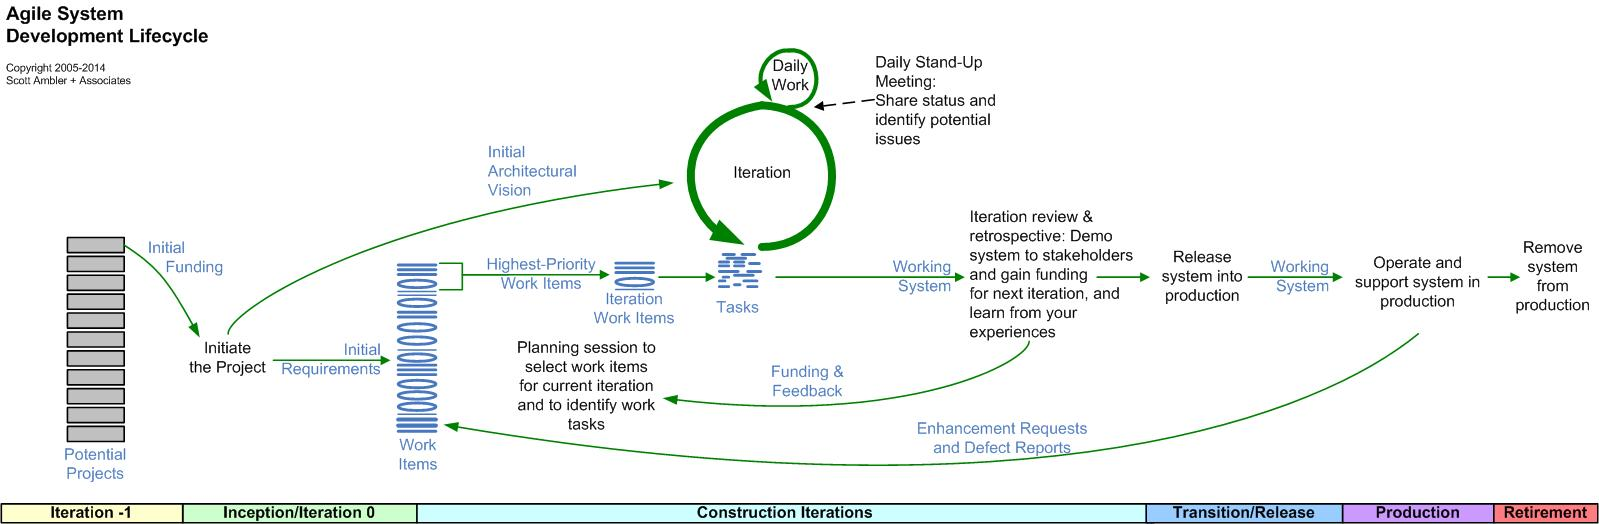
\includegraphics[width=1\textwidth]{softwareengineer/images/agileLifecycleDetailed} 
  \caption{Seleção do ciclo de vida ágil baseado no Scrum \cite{ambysoft:09}}
  \label{fig:scrumlifecycle} 
\end{figure}

\subparagraph{Análise dos Requisitos do Sistema e Análise dos requisitos de software}

\begin{itemize}
  \item Os requisitos serão definidos pelo fornecedor de acordo com as necessidades levantadas pelo adquirente

  \item Todos os requisitos serão definidos e listados no Product Backlog

  \item Eles serão listados e priorizados pelo PO (Product Owner) e Scrum Master antes do Sprint Planning
\end{itemize}

\subparagraph{Projeto de arquitetura do sistema e Projeto de arquitetura do software}

Estas duas atividades são compostas pelos processos de análise de requisitos pelo modelo de ciclo de vida, pois durante as atividades de análise na qual o Product Owner e o cliente geram todas as estórias que seriam os módulos ou casos de uso ou funcionalidades do sistema, parte da equipe técnica se concentrará em definir os requisitos e outra parte em definir como o sistema deveria ser "\textit{montado}". Especialistas em arquitetura de sistemas desenvolveriam modelos arquiteturais que correspondessem as necessidades do projeto ao mesmo tempo em que analistas de negócios e projetistas de sistemas gerariam um projeto modularizado e componentizado montando assim uma arquitetura de como o software deve ser implementado.

\subparagraph{Projeto detalhado do software}

O modelo de ciclo de vida não prioriza o detalhamento em documentação do sistema e sim um modelo de implementação de funcionalidades que tenham sido previamente definidas e que serão complementadas pelas informações constantes do cliente que sempre estará em contato com a equipe.

\subparagraph{Codificação e Teste do software / Integração do software e Integração do sistema}


Isto é um ponto fraco do modelo de ciclo de vida. No Scrum não há definição de papéis na equipe de desenvolvimento, todos são desenvolvedores. Além disso, não há uma definição sobre as atividades de codificação, teste e integração. Neste caso, assumiremos que a empresa de software tem alguns procedimentos e práticas ágeis que a equipe de desenvolvimento deverá seguir. Os procedimentos a serem seguidos pela equipe de desenvolvimento visa otimizar ao máximo o processo de codificação e testes buscando um trabalho que seja auto-organizável e buscando também a formação de uma equipe que se auto-gerencia e se corrija.

O processos de gerenciamento ágil que evidencia os objetivos de foco no desenvolvimento e qualidade
dos testes afim de não gerar retrabalho e falhas futuras do software como:
\begin{itemize}
  \item Programação pareada para funcionalidades complexas e TDD (Test driven development).
  \item Todos os testes devem ser automatizados e executados várias vezes ao dia, com integração contínua;
  \item Comunicação é um fator de extrema importância tratado pelo manifesto ágil\cite{beck2001agile} com muito cuidado. Priorizam a comunicação falada e consequentemente documentada, pois consideram que esta é uma das melhores formas de passagem de conhecimento.
\end{itemize}

O processo de testes também será diferenciado, pois serão realizados dois tipos de testes, que são os unitários e ou automatizados e os testes de integração. Com isso, os erros tornam-se mais facilmente detectáveis e as soluções pra estes se tornam mais rápidas e precisas.

Frente a estas atividades, a integração do software e do sistema torna-se cada vez mais simples, já que todas estas atividades apóiam estas ultimas atividades citadas.






\subparagraph{Teste de qualificação do software e Teste de qualificação do sistema }

O modelo de ciclo de vida não define a atividade de teste e o fator de qualidade de testes do software e do sistema. No entanto, iremos assumir que a empresa adota práticas ágeis que objetivam ter qualidade em seus resultados e por isso sempre mantém o cliente como participante do processo.

\subparagraph{Instalação do software e Apoio à aceitação do software}

O modelo de ciclo de vida não define estas atividades. Neste caso, as práticas adotadas pela empresa será as práticas ágeis. A atividade de aceitação será completamente trabalhada no projeto, pois o principal interessado no projeto mantém-se presente durante todo o processo de entrega de incrementos do sistema, tirando dúvidas dos desenvolvedores realizando reuniões de acompanhamento de entregas como o Sprint Review. Para o processo de instalação assumiremos que os integrantes da equipe de maior conhecimento no sistema junto aos projetistas do sistema e do software são responsáveis junto a seus gerentes pela instalação do sistema, assim conclui-se que existe uma equipe mobilizada para a instalação e a realização da atividade com sucesso.

\begin{table}[htb]
      \begin{center}
        \begin{tabular}{| p{6cm} | l |}
        \hline
        \textbf{Atividade} & \textbf{Cobertura} \\ \hline
        Implementação do processo & Parcial \\ \hline
        Análise dos Requisitos do Sistema e Análise dos requisitos de software & Parcial \\ \hline
        Projeto de arquitetura do sistema e Projeto de arquitetura do software & Não contempla \\ \hline
        Projeto detalhado do software & Não contempla \\ \hline
        Codificação e Teste do software / Integração do software e Integração do sistema & Parcial \\ \hline
        Teste de qualificação do software e Teste de qualificação do sistema & Parcial \\ \hline
        Instalação do software e Apoio à aceitação do software & Parcial \\ \hline
        \end{tabular}
      \end{center}
    \caption{Cobertura das atividades do processo de desenvolvimento}
    \end{table}


\subsubsection{\large{Processo de Operação e Manutenção}}
\label{sec:operacao}

O processo de operação e manutenção ocorrem simultaneamente. O processo de operação consiste em auxilar os usuários no uso do produto recentemente criado \cite{iso12207:95}. A manutenção de software é a atividade durante a qual ocorrem modicações em um ou mais artefatos de software resultante do desenvolvimento de um software (ou de manutenções anteriores), buscando mantê-lo disponível, corrigir suas falhas, melhorar seu desempenho e adequá-lo aos requisitos novos ou modificados, conforme as necessidades de seus usuários\cite{IEEE1990}.

O intuito é que o desenvolvimento seja guiado por testes, sendo que esta prática garante que os erros sejam descobertos rapidamente, com isso, manutenção corretiva é colocada em prática para prevenir ou reduzir a necessidade deste tipo de manutenção depois que o produto foi entregue ao cliente.
Outra prática ágil é o refactoring que garante que uma futura manutenção software possa ser continuada facilmente, auxiliando a categoria de manutenção preventiva e perfectiva.
Outras práticas também auxiliam, como no caso de padrões de desenvolvimento e design simples.

Caso haja uma descontinuação do software, todos os artefatos gerados durante o ciclo de vida do processo de software serão disponibilizados ao cliente, bem como manuais ou qualquer outro documento que o adquirente tenha requisitado em comum acordo.

\begin{table}[htb]
      \begin{center}
        \begin{tabular}{| p{6cm} | l |}
        \hline
        \textbf{Atividade} & \textbf{Cobertura} \\ \hline
        Implementação do processo & Parcial \\ \hline
        Teste operacional & Não contempla \\ \hline
        Operação do sistema & Não contempla \\ \hline
        Suporte ao usuário & Parcial \\ \hline
        \end{tabular}
      \end{center}
    \caption{Cobertura das atividades do processo de operação}
    \end{table}

    \begin{table}[htb]
      \begin{center}
        \begin{tabular}{| p{6cm} | l |}
        \hline
        \textbf{Atividade} & \textbf{Cobertura} \\ \hline
        Implementação do processo & Parcial \\ \hline
        Análise do problema e da modificação & Parcial \\ \hline
        Implementação da modificação & Total\\ \hline
        Revisão/aceitação da manutenção & Parcial \\ \hline
        Migração & Não contempla \\ \hline
        Descontinuação do software & Parcial \\ \hline
        \end{tabular}
      \end{center}
    \caption{Cobertura das atividades do processo de manutenção}
    \end{table}

\section{Requisitos de Software}
\label{sec:requisitos}

A fim de definirmos alguns pontos específicos sobre a área de conhecimento Engenharia de Requisitos de Software, proponho elucidar inicialmente os principais focos a serem seguidos no momento da iniciação desta atividade de Elicitação de Requisitos de Software que é considerada uma atividade de importância em todo o processo de Desenvolvimento do Sistemas. 

De acordo com a norma IEEE Std-830/1998 -IEEE Recommended Practice for Software Requirements Specifications \cite{IEEE830-1998} um conjunto de diretrizes foram definidas para o desenvolvimento de uma ERS que seguem:
\begin{description}
\item [Correção:] Esta característica consiste em observar se todo o requisito que consta do documento é um requisito que reflete uma necessidade real, ou seja, que tenha que ser implementado pelo software;
\item [Não ambiguidade:] Esta característica estabelece que cada um dos requisitos do documento tenha apenas uma interpretação; 
\item [Completude:] Esta característica tem por finalidade analisar se na especificação inclui todos os requisitos significativos, a definição das respostas do software a todos os tipos de dados de entrada em todas as situações possíveis, tanto válidas como inválidas, e referenciam todos os termos, figuras, tabelas, diagramas, além das unidades de medidas empregadas; 
\item[Verificabilidade:] Neste caso, esta característica consiste em verificar se, para cada um dos requisitos contidos no documento, existe um processo finito e economicamente viável por meio do qual uma pessoa ou uma máquina pode checar que o software satisfaz o requisito; 
\item[Consistência:] A finalidade desta característica é observar se nenhum dos requisitos do documento, ao ser verificado individualmente, está em conflito com qualquer outro requisito presente ou contido no mesmo documento; 
\item[Classificação:] O objetivo desta característica é verificar se existem na especificação/documento indicações quanto aos critérios que determinem a importância (essências, condicionais ou opcionais) ou estabilidade do requisito; 
\item[Modificabilidade:] Esta característica consiste em verificar se modificações podem ser realizadas e agregadas ao documento de forma fácil, completa e consistente em relação à  sua estrutura e estilo; 
\item[Rastreabilidade:] A finalidade desta característica está em observar se a origem de cada requisito é clara e se possibilitará alterações e melhorias quando necessário em uma nova versão do produto;
\end{description}

Seguindo estas definições e métricas ao desenvolvimento de uma (ERS) iniciamos o trabalho detalhando com cuidado alguns pontos principais sobre o produto. O Restaurante utilizará o sistema (SGR) que terá entre as suas funcionalidades: padronização das receitas, controle de estoque dos itens utilizados, nas receitas, visibilidade dos garçons quanto à disponibilidade dos itens disponíveis de acordo com o pedido do cliente para determinado prato, controle da disponibilidade das mesas pela recepcionista ou maître, painel informativo sobre pratos concluídos, histórico de consumo dos itens dos últimos 6 meses. O restaurante opera com equipe pequena de funcionários.


\begin{table}[htb]
      \begin{center}
        \begin{tabular}{| p{6cm} | p{6cm} |}
        \hline
        \textbf{O problema de} & Recepção e atendimento manual dos clientes no restaurante, controle manual de entrada e saída de itens do estoque, falta de padronização das receitas das refeições.  \\ \hline
        \textbf{Afeta} & Gino, seus funcionários, fornecedores e clientes. \\ \hline
        \textbf{Cujo impacto é} & O desperdício de insumos, atendimento insatisfatório, perda de receita e erro de provisionamento dos pedidos de compra. \\ \hline
        \textbf{Uma solução de sucesso seria} & Criar um sistema que torne os pedidos de compra precisos, consumo eficiente e controlado dos insumos e aumente a rapidez no atendimento. \\ \hline
        
        \end{tabular}
      \end{center}
    \caption{Declaração do problema}
    \end{table}


\subsection{Atividades e Papéis}

\begin{figure}[H]
  \centering
  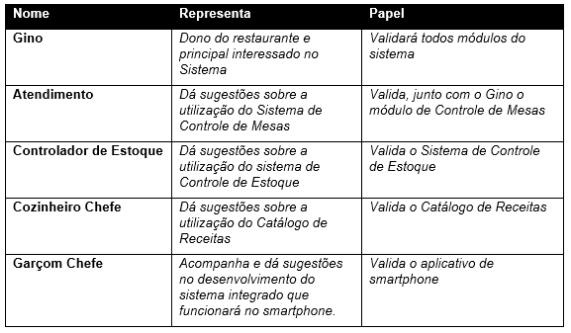
\includegraphics[width=0.8\textwidth]{softwareengineer/images/stakeholders} 
  \caption{Resumo dos stakeholders}
  \label{fig:stakeholders} 
\end{figure}

\begin{figure}[H]
  \centering
  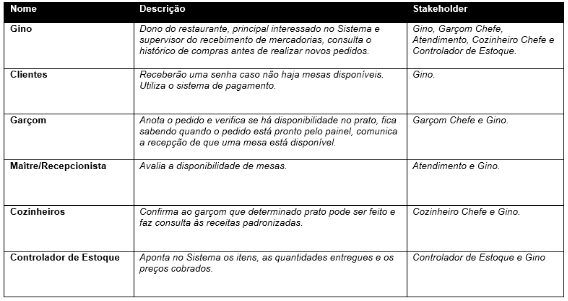
\includegraphics[width=1\textwidth]{softwareengineer/images/users} 
  \caption{Resumo dos usuários}
  \label{fig:users} 
\end{figure}

\subsubsection{Ambiente do usuário}
A equipe do restaurante é composta por dezenove pessoas, sendo destas o dono, oito pessoas da equipe da cozinha (uma destas recebe as mercadorias), oito garçons, um recepcionista e um maître. Se houver crescimento do número de clientes, pode haver contratações de novos funcionários. O restaurante é dividido em cinco ambientes principais: recepção, cozinha, salão de refeição, estoque e escritório.

O restaurante opera em horário de almoço e janta. No almoço serão servidos pratos do dia ou a opção A La Carte. O período de tempo médio de permanência dos clientes no restaurante é de 45 minutos no horário de almoço e 1 hora na janta, podendo variar em finais de semana.

O fluxo de atendimento funciona da seguinte forma: o cliente se apresenta na recepção, a recepcionista verifica se há disponibilidade de mesas de acordo com o número de pessoas. Havendo disponibilidade, o cliente é levado até a mesa onde pode escolher o seu prato. Se não houver disponibilidade, o cliente recebe uma senha impressa que representa um número na fila de espera. No momento que o cliente fizer o pedido, o garçom faz o lançamento do mesmo em um smartphone, que já lhe dá o retorno se há ou não disponibilidade dos ingredientes na cozinha para preparar a solicitação do cliente. 

O garçom pode visualizar através de um painel os pedidos prontos e qual a respectiva mesa. Após o pagamento da conta, os garçons limpam e liberam a mesa informando a recepção.
Quando houver um novo recebimento de mercadoria, Gino e um funcionário irão fazer o lançamento dos itens, quantidades e preços no sistema, a fim de controlar a utilização de insumos. Gino precisa manter um histórico de compras dos últimos seis meses.


Não há nenhum sistema sendo empregado no momento, será um novo estabelecimento.

\begin{figure}[H]
  \centering
  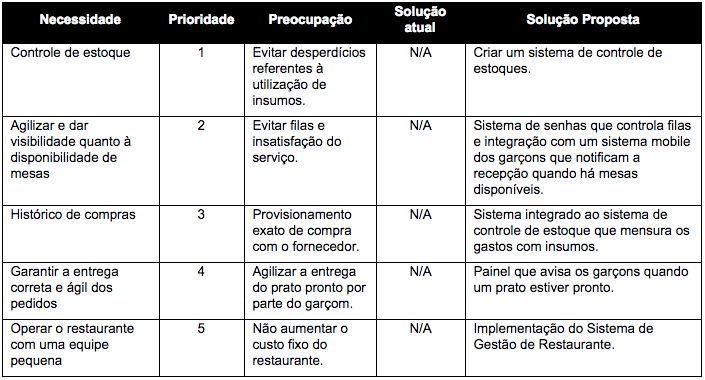
\includegraphics[width=1\textwidth]{softwareengineer/images/stakerholdersneed} 
  \caption{Principais necessidades dos stakeholders e usuários}
  \label{fig:stakerholdersneed} 
\end{figure}

\subsubsection{Visão Geral do Produto}

\subparagraph{Perspectiva do produto}

Todos os módulos compartilharão o mesmo banco de dados.Uma vez que um cliente faça um pedido, o aplicativo integrado do smartphone dos garçons se conectará com o catálogo de receitas que, por sua vez, se conectará com o Sistema de Controle de Estoque e receberá o retorno se há ou não disponibilidade dos ingredientes para preparar o prato solicitado; o Sistema de Controle de Disponibilidade de Mesas se conectará com o aplicativo integrado do smartphone dos garçons para receber a liberação ou ocupação das mesas; o Painel de Pedidos exibirá a mesa e o número do pedido solicitado. Para o pagamento, o sistema SGR será integrado às operadoras de cartão via internet ou 3G, utilizando as máquinas de pagamento padrão.

\subsubsection{Características do produto}

\subparagraph{Sistema de Controle de Estoque}

O controle de estoque fará a gerência dos itens em estoque do restaurante. O usuário deverá cadastrar os produtos descrevendo o item, a quantidade e o valor cobrado pelo item. Conforme houver a necessidade de remover produtos do estoque, um funcionário dará baixa dos itens no sistema, de forma que a cozinha sempre tenha o conhecimento da quantidade de itens disponíveis em estoque, assim como terá um histórico de consumo dos itens disponíveis em estoque.

\subparagraph{Sistema de Controle de Disponibilidade de Mesas}

O recepcionista será o usuário deste sistema e terá um mapa do local que exibe as mesas disponíveis. Caso não hajam mesas disponíveis, o sistema gerará uma senha correspondente a uma fila de espera. Esta senha será impressa e entregue ao cliente.

\subparagraph{Catálogo de Receitas Padronizadas}


O sistema de receitas terá o cadastro de todas as receitas realizadas pelo restaurante, assim como as devidas quantidades de ingredientes e método de preparo. Este sistema terá uma integração com o sistema de controle de estoque no qual o cozinheiro seleciona uma receita e o sistema retorna a informação se há ingredientes disponíveis ou não. Desta forma, a cozinha pode notificar os garçons sobre a indisponibilidade de itens.

\subparagraph{Integração com smartphone}

Os garçons possuirão um smartphone que conterá um aplicativo onde poderão lançar os pedidos dos clientes. É por este aplicativo que os garçons receberão a notificação da cozinha sobre a disponibilidade de pratos e também notificarão a recepção sobre a liberação de mesas.


\subparagraph{Painel de Pedidos}


O painel de pedidos exibirá o número do pedido e a mesa correspondente. Este painel ficará disponível para os garçons.


\subparagraph{Precedência e prioridade}
\begin{enumerate}
  \item Sistema de controle de estoque
  \item Catálogo de receitas
  \item Sistema de controle de disponibilidade de mesas
  \item Integração com smartphone
  \item Painel de pedidos
\end{enumerate}

\subparagraph{Outros requisitos do produto}

Dentre os requerimentos do produto está a aquisição de dois computadores: um para a recepção e outro para o escritório do Gino, com sistema operacional Windows 7 ou superior. O Restaurante deve possuir uma rede de Wi-Fi interna de forma que os computadores possam estar interligados em rede. Cada garçom deverá receber um smartphone com sistema operacional em Android onde será instalado o aplicativo de registro de pedidos. Deverá ser adquirido um painel que exibirá o número da senha de espera dos clientes.

\subsection{Artefatos}

Elicitação de requisitos é a prática de coletar os requisitos de um sistema a partir de informações obtidas do usuário, cliente e stakeholders. 

Elicitação de requisitos não é uma tarefa trivial, pois nunca poderemos afirmar com certeza que todos os requisitos foram coletados pela simples tarefa de perguntar ao cliente como o sistema deve ou não funcionar. As práticas de elicitação de requisitos incluem entrevistas, questionários, observação, workshops, brainstorming, casos de uso, role playing e protótipo.

Antes dos requisitos serem analizados, modelados ou especificados, eles devem ser coletados através de um processo de elicitação. Elicitação de requisitos é parte do processo de engenharia de requisitos.

\subsubsection{Problemas}

O processo elicitação de requisitos pode parecer simples: Pergunte ao cliente, usuário e outras pessoas sobre o objetivo do sistema ou produto, o que deve ser feito, como o sistema se encaixa no negócio, e finalmente, como o sistema será utilizado no dia-a-dia. Porém, problemas podem surgir que complicarão este processo.


Em 1992, Christel e Kang \cite{ChristelIssuesin1992} identificaram problemas que são um desafio para a elicitação de requisitos:

\begin{description}
\item [Problemas de escopo] O escopo do sistema é mal definido ou o cliente/usuário definem detalhes técnicos desnecessários que causam mais confusão, ao invés de simplificar, o objetivo do sistema.

\item [Problema de entendimento] Os clientes/usuários não tem absoluta certeza sobre o que é necessário, tem um pobre conhecimento sobre as capacidades e limitações do ambiente computacional, não tem completo conhecimento do domínio do problema, tem problema de comunicação com os programadores, omitem informações que julgam ser óbvias, especificam requisitos que conflitam com as necessidades do cliente/usuário, ou especifica requisitos intangíveis ou não testáveis.

\item[Problema de volatilidade] Os requisitos mudam com o tempo. A taxa de alteração é mencionado como o nível de volatilidade do requisito.

\end{description}
A qualidade dos requisitos podem ser melhorados através de:

\begin{description}
\item [Visualização] Uso de ferramentas que promovem o melhor entendimento do produto final desejado como visualização ou simulação.
\item [Linguagem consistente] Uso de definições simples e consistentes para descrever os requisitos como uma linguagem natural e uso de termos de negócios comumente utilizados na empresa.

\item [Práticas] Uso sistemático de práticas organizacional que descrevem técnicas de coletar e o tipo de requisitos a serem coletados. Estas práticas devem ser usadas nos projetos da empresa.
\item [Uso de modelos] Produzir um conjunto de modelos e padrões para documentar os requisitos. 
\item [Documentar dependências] Documentar dependências e inter-relações entre os requisitos.
\item [Análise de mudança] Analisar a raiz do problema das alterações nos requisitos e fazer as ações corretivas.
\end{description}

\subsubsection{Técnicas de Elicitação de Requisitos}

O SWEBOK terceira edição \cite{IEEEComputerSociety:2014:GSE:2616205} define as seguintes técnicas de elicitação:

\begin{itemize}
\item Entrevistas (Interviews);
\item Cenários (Scenarios);
\item Protótipos (Prototype);
\item Observação (Observation);
\item Estória de usuário (User stories);
\item Outras técnicas (Other techniques).
\end{itemize}

Selecionar a técnica adequada de elicitação de requisitos não é simples. Para escolher a técnica mais adequada iremos utilizar as seguintes suposições \cite{atil:2012}:

\begin{itemize}
\item É a única técnica que se conhece;
\item A técnica funcionou da última vez, então também funcionará agora;
\item Intuitivamente, conclui-se que a técnica é eficaz na atual circunstância;
\item Alguma metodologia foi adotada, e essa metodologia prescreve uma técnica particular no momento atual.
\end{itemize}

No nosso caso, adotaremos que a empresa tem conhecimento e ampla experiências em estórias de usuário. Esta técnica foi adotada em outros projetos e foi a que obteve maior sucesso. Product Backlog é onde se inicia todo o processo do Scrum, sendo considerada a prática responsável pela parte da elicitação da área de engenharia de requisitos.

Serão realizadas reuniões e serão definidas as estórias de usuário com todos os stakeholders do projeto. Será definido o Product Backlog que é a lista de atividades que serão desenvolvidas no projeto.


\subsubsection{DEFINIÇÃO INCIAL DA LISTA DE PENDÊNCIAS DO PRODUTO DE SOFTWARE (PRODUCT BACKLOG)
}

\subparagraph{Pendências do Produto - ProductBacklog(PB)}

\begin{enumerate}
  \item Sistema de Controle de Estoque
  \item Catálogo de receitas
  \item Sistema de controle de disponibilidade de mesas
  \item Integração com smartphone
  \item Painel de pedidos
\end{enumerate}

\begin{enumerate}
\item \textbf{Sistema de controle de estoque}

\begin{enumerate}
  \item Aceitação do pedido do cliente em relação ao estoque;
  \item Baixa dos itens usados pela cozinha;
  \item Feedback ao catálogo de receitas;
  \item Cadastro dos fornecedores;
  \item Aviso de baixa quantidade de ingredientes em estoque;
  \item Compra de pedido de insumos baseado no histórico dos últimos 6 meses;
  \item Lançamento dos itens no sistema.
\end{enumerate}

\item \textbf{Catálogo de receitas}

\begin{enumerate}
  \item Cadastro de todas as receitas com as respectivas quantidades de ingredientes utilizados;
  \item Indicar se receita será utilizada no almoço, jantar ou ambos;
  \item Indicar se a receita é prato do dia (aumentar quantidade de ingredientes em estoque);
  \item Comparação do pedido do cliente com a quantidade de ingredientes disponíveis em estoque;
  \item Feedback ao garçom.
\end{enumerate}

\item \textbf{Sistema de controle de disponibilidade de mesas}

\begin{enumerate}
  \item Reserva de mesa;
  \item Alocação de mesa;
  \item Desalocação de reserva;
  \item Inserir cliente na lista de espera.
\end{enumerate}

\item \textbf{Integração com smartphone}

\begin{enumerate}
  \item Anotar pedidos;
  \item Desalocação de mesa.
\end{enumerate}

\item \textbf{Painel de pedidos}

\begin{enumerate}
  \item Alterar o status do pedido para “Pronto”.
\end{enumerate}
\end{enumerate}

\subsubsection{Papéis, Responsabilidades e Atributos}

\begin{enumerate}
  \item Gerente

  \begin{enumerate}
    \item Responsabilidades

      \begin{enumerate}
        \item Consulta de produtos em estoque;
        \item Consulta de fornecedores;
        \item Cadastro de fornecedores;
        \item Cadastro de usuários;
        \item Cadastro de receita;
        \item Consulta de balanço por período.
      \end{enumerate}

    \item Atributos

      \begin{enumerate}
        \item Frequência de uso: diária;
        \item Conhecimento excelente do domínio;
        \item Conhecimento excelente de computador;
        \item Controle das operações
      \end{enumerate}
  \end{enumerate}

  \item Garçons

  \begin{enumerate}
    \item Responsabilidades

      \begin{enumerate}
          \item Realizar pedido;
          \item Desalocação de mesas;
          \item Verificar status do pedido;
          \item Encerramento da conta.
      \end{enumerate}

    \item Atributos

      \begin{enumerate}
          \item Frequência de uso: um turno;
          \item Conhecimento do domínio: médio;
          \item Conhecimento de usuário de computador: médio;
          \item Metas gerais de uso: poucas entradas por registro.
      \end{enumerate}
  \end{enumerate}


  \item Cozinheiro

  \begin{enumerate}
    \item Responsabilidades

      \begin{enumerate}
          \item Informa pedido pronto;
          \item Verificar catálogo de receita.

      \end{enumerate}

    \item Atributos

      \begin{enumerate}
          \item Frequência de uso: um turno;
          \item Conhecimento do domínio: bom;
          \item Conhecimento de usuário de computador: bom;
          \item Metas gerais de uso: não entra com registros, apenas pressiona botões.
      \end{enumerate}
  \end{enumerate}

  \item Recepcionista

  \begin{enumerate}
    \item Responsabilidades

      \begin{enumerate}
          \item Verifica disponibilidades de mesa;
          \item Verifica reservas de mesa;
          \item Alocação de mesas;
          \item Incluir reserva.
      \end{enumerate}

    \item Atributos

      \begin{enumerate}
          \item Frequência de uso: período da manhã e tarde;
          \item Conhecimento do domínio: excelente;
          \item Conhecimento de usuário de computador: excelente;
          \item Metas gerais de uso: não entra com registros, apenas pressiona botões.
      \end{enumerate}
  \end{enumerate}

  \item Controlador de estoque

  \begin{enumerate}
    \item Responsabilidades

      \begin{enumerate}
          \item Cadastra novos itens no estoque;
          \item Atualiza quantidade de cada item entregue pelos fornecedores;
          \item Atualiza valor do item entregue.
      \end{enumerate}

    \item Atributos

      \begin{enumerate}
          \item Frequência de uso: uma vez por semana;
          \item Conhecimento do domínio: excelente;
          \item Conhecimento de usuário de computador: excelente;
          \item Metas gerais de uso: entrar com os dados de entrada e saída do estoque, assim como auxiliar o Gino quanto ao relatório de histórico de pedidos.

      \end{enumerate}
  \end{enumerate}

\end{enumerate}

\subsubsection{Estórias de usuário}

\paragraph{Compra de pedido de insumos baseado no histórico dos últimos 6 meses (estoque)}

Eu como um gerente de estoque do restaurante “Da Gino”, quero realizar uma compra de insumo baseado no histórico dos últimos seis meses para suprir o estoque de modo que a realização de novos pedidos pelos clientes não possam ser bloqueados por falta deste suprimento.

\subparagraph{Cenário Principal:}

Seleciona o produto na lista de insumos cadastrados no Sistema e verificar a média de compra.

\subparagraph{Cenário Alternativo:}

Produto desejado não está na lista de produtos cadastrados no sistema.

\subparagraph{Critérios de Aceitação:}

\begin{itemize}
\item Verificar se produto está cadastrado no sistema.
\item Verificar se a quantidade existente no estoque está abaixo do limite.
\item Receber a confirmação com a quantidade do produto requerida para a próxima compra.
\item Cadastrar o produto no sistema e receber confirmação do cadastro com sucesso.
\item Registrar a compra inicial para este produto inserindo a quantidade desejada e receber a confirmação de compra registrada com sucesso.
\end{itemize}

\subparagraph{Teste de Aceitação:}

\begin{itemize}
\item Gerente de estoque insere o produto no campo texto e clica no botão “Procurar Produto”, sistema retorna o produto em uma grid na tela.
\item Gerente de estoque clica sobre o produto encontrado na grid, e uma nova tela é aberta com todas as informações do produto: nome, marca, quantidade em estoque, data da última compra e quantidade comprada.
\item Gerente de estoque clica sobre o botão “Calcular Próxima Compra” e sistema mostra um pop – up com a quantidade requerida para próxima compra e a mensagem “Deseja registrar a nova compra” seguida de dois botões “Sim” e “Não”.
\item Gerente de estoque clica sobre o botão “Sim” e recebe confirmação da compra registrada com sucesso.
\item Gerente de estoque clica sobre o botão “Não” e recebe confirmação da compra não registrada.
\item Gerente de estoque clica sobre o botão “Calcular Próxima Compra” e sistema mostra um pop – up com a mensagem “Suprimento com quantidade suficiente no estoque.”.
\end{itemize}

\subparagraph{Teste Cenário Alternativo:}

\begin{itemize}
  \item Gerente de estoque insere o produto no campo texto e clica no botão “Procurar Produto”, sistema retorna a seguinte mensagem “Produto não encontrado.”.
\item Gerente de estoque clica sobre o botão “Cadastrar Produto” e uma nova tela com um formulário é aberta.
\item Gerente de estoque preenche formulário na nova tela e clica sobre o botão “Salvar” e recebe confirmação “Cadastro do produto realizado com sucesso. ”.
\item Gerente de estoque preenche formulário e clica sobre o botão “Salvar” e recebe alerta “Campos obrigatórios precisam ser preenchidos. ”.
\item Gerente de estoque clica sobre o botão “Registrar primeira compra” e um campo texto é habilitado para inserir informação de quantidade.
\item Gerente de estoque insere um valor de quantidade e clica em “Salvar” e recebe confirmação “Compra inicial registrada com sucesso. ”.
\item Gerente de estoque insere um valor de quantidade e clica em “Salvar” e recebe um alerta “Quantidade inválida ou menor que o limite. ”.

\end{itemize}

\paragraph{Comparar pedido de cliente com estoque (Catálogo de receitas)}

Eu como cozinheiro, eu quero comparar os pedidos com as receitas e com a quantidade de ingredientes em estoque, de tal modo que sistema me avise se está acabando algum ingrediente.

\subparagraph{Cenários Principal:}

Comparação indica que é possível fazer o prato com sucesso.

\subparagraph{Cenário Alternativo:}

Comparação indica que é possível fazer o prato com sucesso, mas um ingrediente está acabando ou acabou.

\subparagraph{Critérios de aceitação:}

\begin{itemize}
\item O sistema compara o pedido do cliente com a receita padronizada e verifica se é possível fazer o prato.  
\item O sistema procura o pedido no catálogo padronizado de receitas e relaciona todos os ingredientes a serem utilizados. 
\item O sistema acessa o estoque e verifica a quantidade itens disponíveis de cada ingrediente. 
\item O sistema indica se algum ingrediente está acabando ou está indisponível.
\end{itemize}

\subparagraph{Teste de aceitação:}

\begin{itemize}
\item O cozinheiro checa o próximo pedido e aperta um botão confirmando que é possível fazer o prato e na tela ou painel de pedidos aparece o status do prato “em andamento”. 
\item Ao termino da confecção do prato, o cozinheiro aperta um botão avisando que o prato está pronto e o sistema muda o  status para “pronto” no painel de pedidos.
\item Aparece piscando, na tela um item de ingrediente que está acabando.
\item Aparece em vermelho,  na tela um item de ingrediente que acabou.
\end{itemize}

\paragraph{Alocação de mesa (Controle de disponibilidade de Mesas)}

Eu, como um recepcionista do Restaurante Da Gino, quero alocar um cliente em uma mesa de forma que no Sistema de Disponibilidade de Mesa, a mesa em questão fique com o status de “Ocupada”.

\subparagraph{Cenários Principal:}

Alocar cliente em uma mesa disponível.

\subparagraph{Cenário Alternativo:}

Alocar cliente em uma mesa ocupada.

\subparagraph{Critério de aceitação:}

\begin{itemize}
\item Alocar um cliente em determinada mesa que antes estava verde no mapa de mesas e ela passa a ficar com a cor vermelha, representando o status de ocupada.
\item Não será possível alocar um cliente em uma mesa com um status vermelho.
\end{itemize}

\subparagraph{Teste de aceitação:}

\begin{itemize}
\item Ao clicar sobre uma mesa vermelha, a seguinte mensagem deve aparecer na tela “Mesa ocupada”;
\item Ao clicar sobre uma mesa verde, a seguinte mensagem deve aparecer na tela “Mesa disponível. \item Deseja alocar um cliente? ”e dois botões de resposta (sim e não).
\item Ao clicar no botão “Sim”, quando perguntado se deseja alocar o cliente, a mesa deverá mudar da cor verde para cor vermelha.
\item Ao clicar no botão “Não”, quando perguntado se deseja alocar o cliente, a mesa deverá permanecer com a cor verde.
\end{itemize}

\paragraph{Anotar Pedido}

Eu como garçom do Restaurante "Da Gino", desejo anotar os pedidos dos clientes no dispositivo móvel com integração com o sistema do restaurante de tal modo que o pedido chegue instantaneamente na cozinha.

\subparagraph{Cenário Principal:}

Anotação do pedido com sucesso.

\subparagraph{Cenário Alternativo:}

Pedido não disponível para solicitação.

\subparagraph{Critérios de aceitação:}

\begin{itemize}
\item Verificar disponibilidade do prato pelos itens da receita.
\item Verificar tempo médio de preparo do prato.
\item Receber confirmação que o pedido foi realizado e está com o status "Em andamento".
\end{itemize}

\subparagraph{Teste de aceitação:}

\begin{itemize}
\item Garçom seleciona uma caixa de checagem dos itens do pedido do cliente, clica no botão 'Realizar pedido', sistema mostra mensagem 'Pedido Confirmado'.
\item Garçom clica no botão 'Realizar Pedido', sistema detecta que nenhum item foi selecionado, sistema mostra mensagem 'Por favor, selecione pelo menos um item'.
\item Garçom seleciona uma caixa de checagemdos itens do pedido do cliente, clica no botão 'Realizar pedido', sistema mostra mensagem 'Item: carne, em falta no estoque'.
\item Garçom seleciona uma caixa de checagemdos itens do pedido do cliente, clica no botão 'Realizar pedido', sistema mostra mensagem 'Pedido não disponível para solicitação'.
\end{itemize}

\paragraph{Alterar status do pedido para "Pronto" (Painel de pedidos)}

Eu como cozinheiro do Restaurante "Da Gino", desejo poder alterar o status dos pedidos solicitados de "Em Andamento" para "Pronto" de tal modo que os garçons visualizem a alteração do status e levem os pratos aos clientes instantaneamente.

\subparagraph{Cenário Principal:}

Status alterado com sucesso.

\subparagraph{Cenário Alternativo:}

Lista de pedidos 'Em Andamento' está vazia.

\subparagraph{Critérios de aceitação:}

\begin{itemize}
\item Verificar pedido com status "Em andamento".
\item Receber confirmação que o status do pedido foi alterado para "Pronto".
\item Verificar se foi dado 'baixa' dos itens do pedido no estoque de acordo com o catálogo de receitas.

\end{itemize}

\subparagraph{Teste de aceitação:}

\begin{itemize}
  \item Cozinheiro seleciona o uma caixa de checagem do pedido a ser alterado o status, clica no botão “Pedidos Prontos”, sistema mostra mensagem “Status do pedido alterado com sucesso”;
\item Garçom clica no botão “Pedidos Prontos”, sistema detecta que nenhum item foi selecionado, sistema mostra mensagem “Por favor, selecione pelo menos um pedido”;
\item Sistema não consegue retornar lista de pedidos “Em Andamento”, exibe mensagem “Não há pedidos em andamento” e botão de atualizar lista.
\item Sistema não consegue retornar lista de pedidos “Em Andamento”, exibe mensagem “Falha ao buscar pedidos em andamento, por favor, tente novamente” e botão de atualizar lista.

\end{itemize}

\section{Qualidade de software}
\label{sec:qualisoftware}


\large{Seção de qualidade de software - Alex}

\subsection{Plano de garantia de qualidade de software}

Definir um plano de garantia de qualidade de software para
o modelo de processo definido em 2.1.3 que esteja em
conformidade com o padrão IEEE Std 730-2002 (ou IEEE
Std 730-2014).

Definir as tarefas de revisão deverão utilizar o IEEE Std
1028-2008:IEEE Standard for Software Reviews and Audits.

\subsection{Tarefas e papéis}

Detalhar as tarefas do plano de garantia de qualidade de
software definido no item anterior. Detalhar também os
papéis dos responsáveis envolvidos.

Definir os artefatos produzidos pelas tarefas e dar um
exemplo de artefato.



\section{Gerência da engenharia de software}
\label{sec:gerenciaengenharia}

\large{Seção gerência de engenharia de software - alex}

Assumir o modelo de processo de software e o plano de garantia
de qualidade de software definidos em 2.1.3 e 2.3.1.

\subsection{Estimativa do projeto}

Aplicar uma técnica de estimativa para o projeto do
exemplo da disciplina, explicando os detalhes desta
aplicação

Justificar a escolha, determinar os objetivos da estimativa e
discutir os resultados da estimativa.

\subsection{Planejamento do projeto}

Apresentar um esboço do planejamento do projeto
consistente com os resultados da estimativa acima e os
modelos e planos adotados em todo o trabalho.



\section{Gerência de configuração de software}
\label{sec:gerenciaconfig}

Gerência de configuração de software, gerência de configuração ou ainda gestão de configuração de software é uma área da engenharia de software responsável por fornecer o apoio para o desenvolvimento de software. Suas principais atribuições são o controle de versão, o controle de mudança e a auditoria das configurações. Roger Pressman, em seu livro Software Engineering: A Practitioner's Approach, especifica que a gerência de configuração de software (GCS) é o:

\begin{quote}
“conjunto de atividades projetadas para controlar as mudanças pela identificação dos produtos do trabalho que serão alterados, estabelecendo um relacionamento entre eles, definindo o mecanismo para o gerenciamento de diferentes versões destes produtos, controlando as mudanças impostas, e auditando e relatando as mudanças realizadas."
\end{quote}

\subsection{Plano de gerência de configuração de software}

\subsubsection{Introdução}

O Plano de Gerência de Configuração apresenta todas as tarefas do Gerenciamento de Configuração e mudanças no projeto, para garantir a sua integridade e o mantendo o domínio das mudanças ocorridas durante o desenvolvimento. 

\paragraph{Definições, Acrônimos e Abreviações}

Segue as definições utilizadas no plano de gerência de configuração:

\begin{table}[H]
      \begin{center}
        \begin{tabular}{| l | l |}
        \hline
        \textbf{Termo} & \textbf{Significado} \\ \hline
        Scrum & Metodologia ágil para gestão e planejamento de projetos de software \\ \hline
        RUP & Rational Unified Process \\ \hline
        IDE & Ambiente de Desenvolvimento Integrado \\ \hline
        GC & Gerência de Configuração \\ \hline
        CCM & Comitê para o Controle de Mudanças \\ \hline
        SM & Solicitação de mudança \\ \hline
        Baseline & Conjunto de itens de configuração que conseguiram um estado comprovado de estabilidade. \\ \hline
        \end{tabular}
      \end{center}
    \caption{Definições, Acrônimos e Abreviações}
    \end{table}

\subsubsection{Gerenciamento de Configuração de Software}

\paragraph{Organização, Responsabilidades e Interfaces} 

No Scrum não tem perfil definido para Gerente de Configuração. Em contrapartida, o Scrum Team deve executar todo o trabalho necessário para concluir a Sprint, incluindo as atividades de gerência de configuração.

No modelo tradicional de desenvolvimento, o gerente de configuração é a parte central do processo de desenvolvimento. Ele é responsável pelo trabalho de deploy, verificar se os artefatos estão sob controle, verifica se todas partes corretas do sistema foram incluídas na versão.

No Scrum, as atividades diárias de um gerente de configuração é separado em partes para membros do time. Uma parte é executada pelo Product Owner e outra parte é executada pelo Scrum Team (e talvez uma parte pelo Scrum Master).

No nosso caso, o gerente de configuração será um membro permanente do time. Ele irá ser o expert em gerência de configuração, porém irá contribuir também no projeto (design), nos testes, código-fonte, documentação - tudo que é necessário para alcançar o objetivo da Sprint. Ele irá educar os outros membros do time para aprenderem a fazer o deploy e build do sistema.

\paragraph{Artefatos da Gerência de Configuração x Atividades da Gerência de Configuração} 

As atividades da Gerência de Configuração estão definidas no IEEE Std 828-2012 \cite{6170935} e são divididas em GCOs, que serão abrangidos e controlados nos artefatos gerados. Como o Scrum não contempla soluções nesta área explicitamente, adaptações foram feitas para que a gerência de configuração fosse implementada no processo.

\begin{table}[H]
      \begin{center}
        \begin{tabular}{| l | l |}
        \hline
        \textbf{Artefatos} & \textbf{Atividades} \\ \hline
        Plano de Configuração & GCO1, GCO2 \\ \hline
        Repositório organizado para os Itens de Configuração & GCO1, GCO2, GCO3, GCO5 \\ \hline
        Baselines & GCO3 \\ \hline
        Banco de dados de Requisições de Mudança (Issues) & GCO4, GCO5 \\ \hline
        Relatórios de Auditorias da Configuração & GCO5, GCO6, GCO7 \\ \hline
        \end{tabular}
      \end{center}
    \caption{Artefatos da Gerência de Configuração x Atividades da Gerência de Configuração}
    \end{table}
 
  

 \subsubsection{Identificação da Configuração}

 \paragraph{Métodos de Identificação}

 Todos os artefatos gerados, com exceção de código fonte, neste projeto terão a seguinte nomenclatura:

\begin{myprop}
\textit{DaGino\_<TEXTO\_LIVRE> - <TIPO\_ART>.<EXT>}
\end{myprop}


\begin{table}[H]
      \begin{center}
        \begin{tabular}{| l | p{6cm} |}
        \hline
        \textbf{Identificador} & \textbf{Descrição} \\ \hline
        **<TEXTO\_LIVRE>** (Não obrigatório) & Texto livre que identifique unicamente o arquivo. Ex.: Reunião 01. \\ \hline
        **<TIPO\_ART>** & Tipo do artefato. Ex: Ata, EAP, Diagrama de Caso de Uso, etc. \\ \hline
        **<EXT>** & A extensão do arquivo. Ex.: doc, xls, java, etc. \\ \hline
        \end{tabular}
      \end{center}
    \caption{Métodos de Identificação}
    \end{table}

\paragraph{Baselines do Projeto}

Para que se dê a criação de uma baseline, é necessário que o gerente de configuração faça uma Auditoria de Configuração primeiro e autorize a criação dessa baseline, haja vista que o mesmo estará envolvido em todas as etapas do projeto, sendo este responsável por preparar o ambiente em que os artefatos serão versionados.

\subparagraph{Tag}

As baselines, quando criadas, conterão todo o repositório Git, incluindo código fonte, diagramas, atas de reunião, etc. e serão numeradas com o seguinte formato, a partir do número 0 (zero):

\begin{myprop}
<major>.<minor>.<patch>
\end{myprop}

E serão construídas com as seguintes orientações:

Quebra de compatibilidade com versões anteriores, avança o <major>.
Adição de novas funcionalidades sem quebrar compatibilidade com versões anteriores, avança o <minor>.
Correção de bugs e outras alterações, avança <patch>.
Adotaremos como referência o site do semver na Internet \url{https://semver.org/}.

\subparagraph{Notas de release}

Ao criar uma nova baseline no GitHub, há opção de colocar notas de release e anexar um arquivo executável do projeto em questão. Por exemplo, no aplicativo utilizado no serviço de refeição pelos garçons, um arquivo .apk construído a partir do código fonte do dado baseline pode ser o anexo, e as notas de release deverão ser feitas juntamente com a equipe de Manutenção de Software em texto na linguagem Markdown no seguinte esqueleto:

\begin{myprop}
\#\#\# Histórico de mudanças \\
- *[Novo: (...)]* \\
- *[Correção: (...)]* \\
- *[Melhoria: (...)]* \\
- *[Menor: (...)]* 
\end{myprop}

A ordem das categorias de mudanças devem ser obedecidas conforme texto acima. Caso o aplicativo do serviço de refeição venha a ser hospedado na loja de aplicativos da Google, a Play Store, as mesmas notas de release poderão ser usadas ao publicar novas atualizações do aplicativo.

\subsubsection{Estrutura do Repositório de Versões}

O GitHub é uma plataforma de hospedagem de projetos de software que oferece, além de armazenamento de repositórios GIT e/ou SVN, uma área do repositório específica para documentação online (Portal Wiki) e outra para controlar tarefas e mudanças no projeto (issues). A fim de se ter melhor aproveitamento da plataforma e agilidade no ciclo de vida Scrum do projeto do Restaurante \textit{Da Gino}, todos os artefatos de software e o gerenciamento do projeto será feito no GitHub e/ou em ferramentas integradas ao GitHub.

\paragraph{Repositório principal}

O repositório do aplicativo do serviço de refeição \textit{Da Gino}, podendo ser controlado pelo sistema de controle de versão GIT ou SVN, deve ter os seguintes artefatos nos respectivos diretórios relacionados abaixo (em ordem alfabética):

\begin{table}[H]
      \begin{center}
        \begin{tabular}{| l | p{6cm} |}
        \hline
        \textbf{Diretório} & \textbf{Conteúdo} \\ \hline
        . & README do repositório \\ \hline
        DaGinoSerRef & Código fonte com Javadoc - projeto do Android Studio \\ \hline
        ./reuniões & Atas de reuniões em formato Markdown (.md) \\ \hline
        Processo & Documento em PDF do Processo de Desenvolvimento de Software da empresa fictícia IPTec \\ \hline
        Projeto & Projeto Diretório relacionado à artefatos diversos do projeto. \\ \hline
        ./anexos & Arquivos de imagem de itens exportados: Diagrama de Caso de Uso do \textit{DaGino}; Diagrama de Classes; Diagrama de Componentes; Diagrama de Implantação; Referências das imagens dos diagramas - README \\ \hline
        ./anexos/ciclo de vida & Arquivos de imagem do Ciclo de Vida do projeto \\ \hline
        ./anexos/registros de aprovação & Arquivos de imagem com assinaturas à mão de integrantes da equipe \\ \hline
        ./anexos/ciclo de vida & Arquivos de imagem do Ciclo de Vida do projeto \\ \hline
        ./anexos/ciclo de vida & Arquivos de imagem do Ciclo de Vida do projeto \\ \hline
        ./extra & Itens diversos relacionados ao projeto que não se encaixa em nenhuma das categorias montadas no repositório: Fotos, Vídeos, Apresentações, etc.: Protótipo de Interface Gráfica (GUI) do aplicativo \\ \hline
        \end{tabular}
      \end{center}
    \caption{Repositório principal}
    \end{table}

\paragraph{Repositório de documentação (Wiki)}

O Wiki do \textit{Da Gino}, controlado apenas por GIT e pelo GitHub de forma online, não tem divisão por diretórios, pelo fato de que este repositório tem apenas arquivos de texto na linguagem de marcação Markdown (.md) convertidos automaticamente para páginas HTML pelo GitHub para exibição online no navegador de Internet. Como o GitHub cria uma abstração de que é um website a documentação do repositório, não é exibido o formato de hierarquia de arquivos e pastas como no repositório principal.

Para estruturação do Wiki, a página principal (Home) e a barra lateral do Wiki terão a divisão feita por "Portais", a exemplo dos Portais do Wikipédia, mas para áreas de conhecimento da Engenharia de Software aplicadas no projeto:


\begin{table}[H]
      \begin{center}
        \begin{tabular}{| l | p{6cm} |}
        \hline
        \textbf{Gerência de Projeto} & \textbf{Documentação relacionada ao gerenciamento do projeto} \\ \hline
        Planejamento & Plano de projeto \\ \hline
        Procedimentos & Relatórios de Monitoramento \\ \hline
        \end{tabular}
      \end{center}
    \caption{Gerência de projeto}
    \end{table}

  

\begin{table}[H]
      \begin{center}
        \begin{tabular}{| l | p{6cm} |}
        \hline
        \textbf{Gerência de Configuração} & \textbf{Documentação relacionada ao gerenciamento de itens de configuração do projeto} \\ \hline
        Planejamento & Plano de Gerência de Configuração \\ \hline
        Procedimentos & Relatórios de Auditorias de Configuração \\ \hline
        \end{tabular}
      \end{center}
    \caption{Gerência de configuração}
    \end{table}

\begin{table}[H]
      \begin{center}
        \begin{tabular}{| l | p{6cm} |}
        \hline
        \textbf{Engenharia de Requisitos} & \textbf{Documentação relacionada aos artefatos de elaboração do produto em alto nível} \\ \hline
        Planejamento & Documento de Especificação de Objetivos e Requisitos (EOR) \\ \hline
        \end{tabular}
      \end{center}
    \caption{Engenharia de requisitos}
    \end{table}

 

\begin{table}[H]
      \begin{center}
        \begin{tabular}{| l | p{6cm} |}
        \hline
        \textbf{Verificação e Validação (V\&V)} & \textbf{Documentação relacionada às atividades de V\&V no projeto} \\ \hline
        Planejamento & Plano de Verificação e Validação \\ \hline
        Procedimentos & Documento de Procedimentos (para cada artefato escolhido no Plano para passar por V\&V - exceto Planos Gerenciais); Relatório de Resultados (para cada artefato escolhido no Plano para passar por V\&V - exceto Planos Gerenciais) \\ \hline
        \end{tabular}
      \end{center}
    \caption{Verificação e Validação}
    \end{table}


    \begin{table}[H]
      \begin{center}
        \begin{tabular}{| l | p{6cm} |}
        \hline
        \textbf{Manutenção} & \textbf{Documentação relacionada às atividades de Manutenção de software no projeto} \\ \hline
        Planejamento & Plano de Manutenção \\ \hline
        \end{tabular}
      \end{center}
    \caption{Verificação e Validação}
    \end{table}

    \begin{table}[H]
      \begin{center}
        \begin{tabular}{| l | p{6cm} |}
        \hline
        \textbf{Garantia da Qualidade} & \textbf{Documentação relacionada às atividades de Garantia da Qualidade no projeto} \\ \hline
        Planejamento & Plano de Garantia da Qualidade \\ \hline
        Procedimentos & Relação de não conformidades (para cada Plano Gerencial escolhido no Plano de GQA para passar por Avaliação); Relatório de Avaliação (para cada Plano Gerencial escolhido no Plano de GQA para passar por Avaliação) \\ \hline
        \end{tabular}
      \end{center}
    \caption{Verificação e Validação}
    \end{table}


    \begin{table}[H]
      \begin{center}
        \begin{tabular}{| l | p{6cm} |}
        \hline
        \textbf{Templates} & \textbf{Modelos de documentos diversos para uso em todo o repositório do projeto} \\ \hline
        Gerência de Projeto & Plano de Projeto; Relatório de Monitoramento; Agenda de Reunião; Ata de Reunião \\ \hline
        Gerência de Configuração & Plano de Gerenciamento de Configuração; Auditoria de Configuração \\ \hline
        Engenharia de Requisitos & Documento de Especificação de Objetivos e Requisitos (EOR) \\ \hline
        Verificação e Validação (V\&V) & Plano de Verificação e Validação; Documento de Procedimentos; Relatório de Resultados \\ \hline
        Manutenção & Plano de Manutenção; Documento de Solicitação de Mudança; Documento de Análise de Viabilidade e Riscos; Documento de Controle e Correção; Notas de Release; Documento de Migração \\ \hline
        Garantia da Qualidade & Plano de Garantia da Qualidade; Relatório de avaliação; Relação de não conformidades \\ \hline
        \end{tabular}
      \end{center}
    \caption{Verificação e Validação}
    \end{table}

\subsubsection{Controle de Configuração e Mudança}

\paragraph{Processamento e Aprovação de Solicitações de Mudança}

O repositório é mantido e controlado pelo Scrum Team. A plataforma de Issues do GitHub é aonde serão feitas e registradas todas as atividades em relação à mudanças no software. As mesmas issues podem ser visualizadas na ferramenta de Gerenciamento de Projetos waffle.io \url{https://waffle.io/}.

Quando alguém cria uma nova issue (reporta um bug, solicita uma nova funcionalidade), é feita uma análise de viabilidade e riscos. Se a mudança solicitada não é viável, é informada ao autor da solicitação a inviabilidade e é fechada a issue; caso contrário, os Mantenedores planejam e executam a mudança e o Gerente de Configuração e o de Verificação e Validação monitoram o procedimento. Caso a mudança feita tenha sido um sucesso (revisada), o gerente de configuração prepara mais uma release (baseline) do software.

\paragraph{Comitê de Controle de Mudança (CCB)}

No Scrum, não há Comitê de Controle de Mudança como no modelo tradicional de GCM.

As solicitações de mudança do Product Backlog são discutidos, priorizados, e decidido pelo Product Owner na reunião do Sprint Planning. O Scrum Team escolhe os itens do topo e adicionam no Sprint Backlog. A quantidade de itens é baseado no tamanho da Sprint e complexidade das mudanças/funcionalidades. No caso do Scrum, o Comitê de Controle de Mudança é mais "\textit{light}". As mesmas atividades estão presentes incluindo análise, coordenação, aprovação, reprovação, porém é menos formal.

Um Template para issue de Solicitação de Mudança (SM) está disponível no Wiki do GitHub para padronizar as informações necessárias para uma solicitação de mudança.

A solicitação de mudança (SM) deve ser deve ser registrada nas Issues do GitHub, assim como as Análises de Viabilidade e Riscos e o Planejamento de mudanças, disponível no repositório do projeto. Algumas informações são necessárias para a devida criação do solicitação.

\subsubsection{Estimativa do Status de Configuração}

\paragraph{Processo de Armazenamento de Mídia e Liberação do Projeto}

O repositório do projeto deverá ser "clonado" por todos os integrantes da equipe.

\paragraph{Relatórios e Auditorias}

A auditoria é feita durante a reunião de Sprint Review. O Spring Backlog contém todos os itens necessários a entrega e caso o ciclo seja de 2 a 4 semanas, a lista é normalmente pequena.
O time demonstra cada estória no Sprint Backlog para o Product Owner e ele (ela) pode ver se o item satisfaz os requisitos. Portanto, a auditoria de configuração é feita de forma informal e pessoalmente.

\subsubsection{Marcos}

Os principais marcos do projeto são os de último dia de sprint, em que há a criação da baseline do repositório de controle de versão e a realização das cerimônias de final de sprint do Scrum. 

O Plano de Gerência de Configuração é alterado nos seguintes casos:

\begin{itemize}
\item O repositório de versões não está atendendo as necessidades dos integrantes da equipe;
\item O Plano não foi aprovado pela V\&V e precisa ser refatorado.
\item Quando for necessária a refatoração deste Plano, deve ser criada uma nova issue de solicitação de mudança no Plano de GCS.
\end{itemize}

\subsubsection{Treinamento e Recursos}

\begin{itemize}
\item No README do repositório principal há um guia rápido para utilização do sistema de controle de versão Git;
\item No site do GitHub há um tutorial iterativo para aprender a usar o Git em 15 minutos, criado pelo Code School: \url{https://try.github.io}
\item A documentação online do Git tem diversos conteúdos a respeito de controle de versão e gerência de configuração de forma completa, mas didática: \url{http://git-scm.com/doc}
\item Nos guias online do GitHub tem um guia rápido para aprendizagem da linguagem de marcação Markdown: \url{https://guides.github.com/features/mastering-markdown/}
\end{itemize}


\subsection{Tarefas e papéis}

Descrever as tarefas da gerência de configuração do plano
definido no item anterior. Descrever também os papéis dos
responsáveis envolvidos.

Definir os artefatos produzidos pelas tarefas e dar um
exemplo de artefato.



\section{Teste de software}
\label{sec:teste}

\subsection{Padrão para o Teste de Aceitação}

Adaptando a citação de Glen Myers \cite{Myers:2004:AST:983238} pode-se dizer que a atividade de teste de software é o processo de revisar especificações, projetos e programas com a intenção de descobrir erros. Alguns dos itens que são comuns a todos autores e pesquisadores do assunto teste de software e que descrevem os fundamentos e princípios desta atividade estão relacionados abaixo:

\begin{itemize}
\item Conforme a Lei de Pareto, 80\% dos erros podem ser localizados em 20\% do projeto, geralmente nos módulos principais do sistema;

\item A atividade de teste não prova a ausência de erros, apenas a existência dos mesmos;
\item Bons casos de teste são aqueles que encontram falhas no sistema até então não descobertas;
\item Bons casos de teste são projetados levando em conta os requisitos do projeto;
\item Um critério que pode ser utilizado para determinação do esforço a ser gasto na atividade de teste de software é verificar qual o grau de severidade das conseqüências advindas do seu mau funcionamento;
\item A probabilidade de encontrar um erro numa determinada parte do sistema é proporcional ao número de erros já encontrados nesta parte;
\item O nível de esforço previsto para testes deve levar em consideração a integridade do projeto, a integridade, criticidade, o custo por mal funcionamento, os requisitos de qualidade e acurácia especificados.
\item A maior parte dos autores concorda que os programas devem, preferencialmente, ser testados por pessoas não envolvidas no processo de desenvolvimento, mas sim por uma equipe independente. Pode haver também a interação dos desenvolvedores com a equipe independente, justificando as decisões tomadas durante o projeto. Esta abordagem ajuda na revisão do projeto.

\end{itemize}

O objetivo da atividade de teste pode ser entendido da seguinte forma:

\begin{itemize}
\item no início de cada fase verificar se esta etapa do projeto reflete exatamente os requisitos e definições da fase imediatamente anterior, para com isso garantir que o produto encomendado e o gerado pela atividade de desenvolvimento do software será o mesmo através dos diferentes níveis de refinamento do projeto;
\item verificar se não existem erros de lógica no projeto e código, no fluxo de dados, no entendimento de requisitos, de codificação, tipográficos ou de interface em todas as fases do projeto;
\item identificar e interferir na presença do erro, iniciando-se a depuração, sendo que quanto antes for descoberta a falha, menos custoso será para adequá-la;
\item ter em mente que, uma vez que errar é humano e atividade de desenvolvimento de software é um exercício bastante complexo, os erros existem e devem ser descobertos, portanto o sucesso em um teste consiste em descobrir os erros e corrigi-los.
\end{itemize}

\subsubsection{Configurando o uso da norma IEEE Std 829-2008 \cite{IEEE829}}

De acordo com a apresentação da aula 10.

\paragraph{Níves de integridade}

Definição de um conjunto de características do sistema selecionadas como importantes para as partes interessadas, ajudam a definir os níveis de controle de qualidade a ser aplicado no desenvolvimento e/ou entrega do produto de software.

\begin{figure}[H]
  \centering
  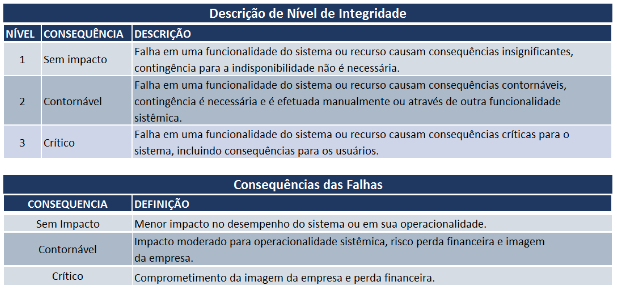
\includegraphics[width=1\textwidth]{softwareengineer/images/integrity-level} 
  \caption{Descrição de nível de integridade}
  \label{fig:integrity} 
\end{figure}

\paragraph{Master Plan}

Identificação e breves explanações sobre os esforços de teste e suas finalidades, a serem detalhados em cada LTP (Level Test Plan), assim explicação do esforço de procedimentos de testes regressivos e testes de inspeção de código automatizados.

\begin{figure}[H]
  \centering
  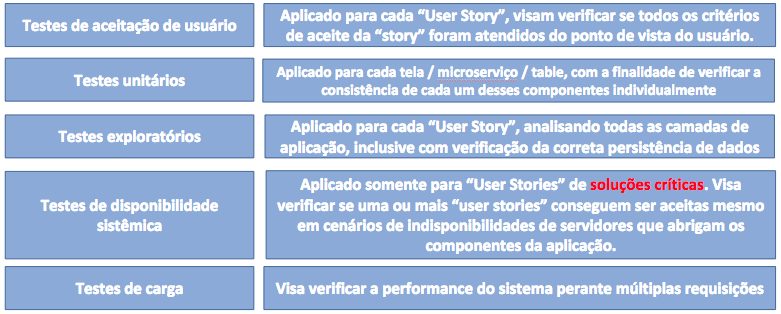
\includegraphics[width=1\textwidth]{softwareengineer/images/master-plan} 
  \caption{Master Plan}
  \label{fig:masterplan} 
\end{figure}

A matriz de integridade e plano de teste adotado segundo a apresentação da aula 10.

\begin{figure}[H]
  \centering
  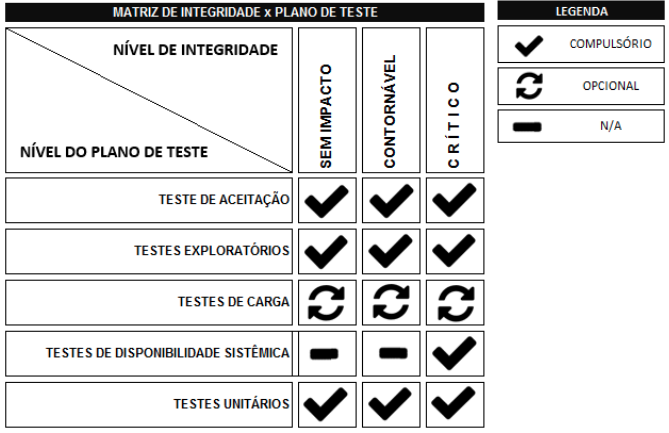
\includegraphics[width=0.8\textwidth]{softwareengineer/images/matrix-integrity} 
  \caption{Matriz de integridade X Plano de teste}
  \label{fig:matrix-integrity} 
\end{figure}

\subsubsection{Níveis de integridade e sua aplicação para cada solução do sistema “\textit{Da Gino}”}

Para cada solução do restaurante \textit{Da Gino} e de acordo com a matriz de integridade e plano de teste, temos o seguinte quadro:

\begin{figure}[H]
  \centering
  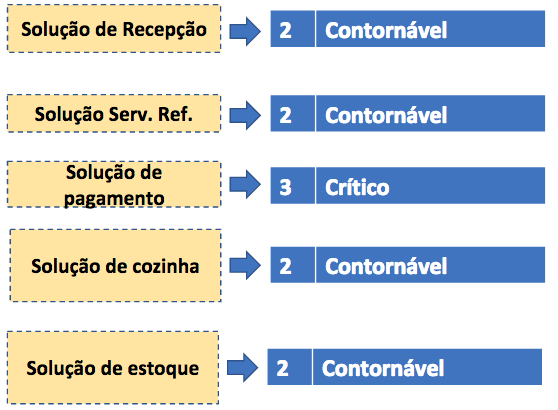
\includegraphics[width=0.6\textwidth]{softwareengineer/images/da-gino-integrity-level} 
  \caption{Níveis de integridade e sua aplicação}
  \label{fig:da-gino-integrity-level} 
\end{figure}

Abaixo uma visão geral dos testes no processo de desenvolvimento:

\begin{figure}[H]
  \centering
  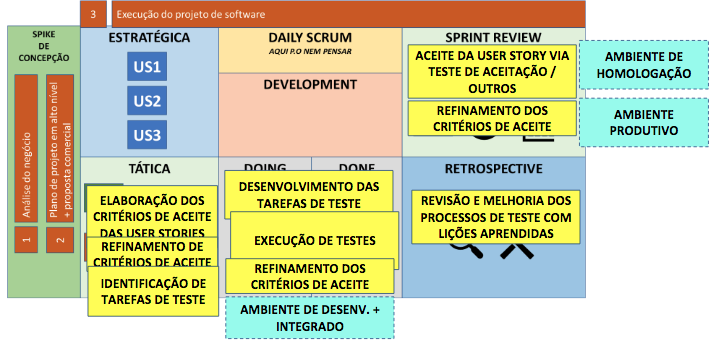
\includegraphics[width=1\textwidth]{softwareengineer/images/model-cycle-tests} 
  \caption{Visão geral dos testes na execução do projeto}
  \label{fig:model-cycle-tests} 
\end{figure}

Segue as responsabilidades de acordo com o nosso modelo de desenvolvimento:

\begin{figure}[H]
  \centering
  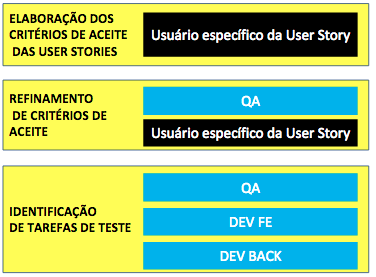
\includegraphics[width=0.6\textwidth]{softwareengineer/images/responsibilities-1} 
  \caption{Responsabilidades - Figura 1}
  \label{fig:responsibilities-1} 
\end{figure}

\begin{figure}[H]
  \centering
  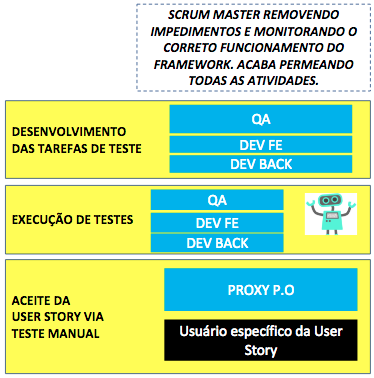
\includegraphics[width=0.6\textwidth]{softwareengineer/images/responsibilities-2} 
  \caption{Responsabilidades - Figura 2}
  \label{fig:responsibilities-2} 
\end{figure}

\begin{figure}[H]
  \centering
  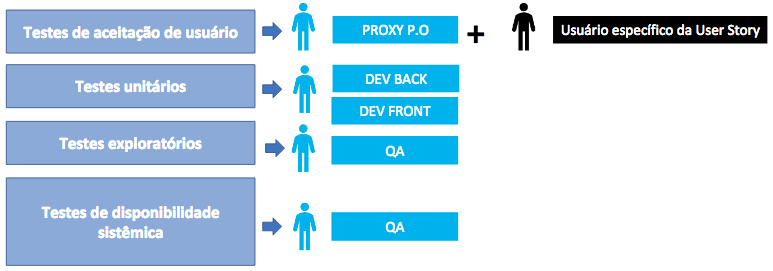
\includegraphics[width=0.8\textwidth]{softwareengineer/images/responsibilities-3} 
  \caption{Responsabilidades - Figura 3}
  \label{fig:responsibilities-3} 
\end{figure}






\subsection{Definição do Teste de Aceitação}

\begin{enumerate}
  \item Recepção ao cliente
  \item Serviço de refeição
  \item Cozinha
  \item Pagamento
  \item Estoque
\end{enumerate}

\begin{enumerate}


\item \textbf{Recepção ao cliente}

\begin{enumerate}
  \item Reserva de mesa;
  \item Alocação de mesa;
  \item Desalocação de reserva;
  \item Inserir cliente na lista de espera.
\end{enumerate}

\item \textbf{Serviço de refeição}

\begin{enumerate}
  \item Anotar pedidos;
  \item Desalocação de mesa.
\end{enumerate}


\item \textbf{Cozinha}

\begin{enumerate}

  \item Recebe pedidos registrados pelos garçons;
  \item Atualiza estoque;
  \item Organiza pedidos;
  \item Libera pedido para cozinheiro;
  \item Prepara os pratos em ordem conforme registro do pedido;
  \item Disponibiliza para servir;
  \item Cadastro de todas as receitas com as respectivas quantidades de ingredientes utilizados;
  \item Indicar se receita será utilizada no almoço, jantar ou ambos;
  \item Indicar se a receita é prato do dia (aumentar quantidade de ingredientes em estoque);
  \item Comparação do pedido do cliente com a quantidade de ingredientes disponíveis em estoque;
  \item Feedback ao garçom.
\end{enumerate}

\item \textbf{Pagamento}

\begin{enumerate}
  \item Cálculo do total da conta
  \item Registro por tipo de pagamento
\end{enumerate}

\item \textbf{Estoque}

\begin{enumerate}
  \item Aceitação do pedido do cliente em relação ao estoque;
  \item Baixa dos itens usados pela cozinha;
  \item Feedback ao catálogo de receitas;
  \item Cadastro dos fornecedores;
  \item Aviso de baixa quantidade de ingredientes em estoque;
  \item Compra de pedido de insumos baseado no histórico dos últimos 6 meses;
  \item Lançamento dos itens no sistema.
\end{enumerate}
\end{enumerate}

\subsubsection{Papéis, Responsabilidades e Atributos}

\begin{enumerate}


  \item \textbf{Recepção ao cliente}

    \begin{enumerate}

      \item Recepcionista

      \begin{enumerate}
        \item Responsabilidades

          \begin{enumerate}

            \item Recepciona os clientes
            \item Consulta ocupação da mesa
            \item Realiza registro de ocupação da mesa
            \item Conduz cliente até a mesa
          \end{enumerate}

        \item Atributos

          \begin{enumerate}
            \item Frequência regular de uso na primeira hora após abertura do restaurante para os clientes às 11:00 a.m primeira hora aprx. 70 clientes;
            \item Alta frequência de uso entre os horários  das 12:00 p.m até às 15:00 p.m, entre 130 e 180  clientes;
            \item Bom conhecimento no domínio de interesse.
            \item Ótimo conhecimento em computadores e mobile.
            \item Muitas consultas e poucas entradas de dados.
          \end{enumerate}
      \end{enumerate}

      \item Responsável de reservas

      \begin{enumerate}
        \item Responsabilidades

          \begin{enumerate}
            \item Realiza o registro de reservas
            \item Administra calendário de reservas pelo telefone
          \end{enumerate}

        \item Atributos

          \begin{enumerate}

            \item Frequência de utilização regular durante horário comercial;
            \item Ótimo conhecimento em computadores e mobile;
            \item Bom conhecimento do domínio.
            \item Poucas entradas de dados;
            \item Muitas consultas;
          \end{enumerate}
      \end{enumerate}

    \end{enumerate}

\item \textbf{Cozinha}

    \begin{enumerate}

      \item Auxiliar

      \begin{enumerate}
        \item Responsabilidades

          \begin{enumerate}
            \item Recebe pedidos  registrados pelos garçons
            \item Atualiza estoque
            \item Organiza pedidos
            \item Libera pedido para cozinheiro.
          \end{enumerate}

        \item Atributos

          \begin{enumerate}
            \item Alta frequência de utilização durante horário comercial;
            \item Ótimo conhecimento do domínio de interesse;
            \item Habilidade regular com computadores e mobile;
            \item Muitas entradas de dados;
            \item Muitas consultas;
            \item Alta interação interdisciplinar;
          \end{enumerate}
      \end{enumerate}

      \item Cozinheiro

      \begin{enumerate}
        \item Responsabilidades

          \begin{enumerate}
            \item Prepara os pratos em ordem conforme registro do pedido 
            \item Disponibiliza para servir.
          \end{enumerate}

        \item Atributos

          \begin{enumerate}
            \item Alta frequência de utilização durante os horários das 11:00 a.m às 15:00 p.m
            \item Ótimo conhecimento do domínio de interesse;
            \item Baixa habilidade com computadores e mobile;
            \item Nenhuma entrada de dado;
            \item Muitas consultas;
          \end{enumerate}
      \end{enumerate}

    \end{enumerate}

\item \textbf{Estoque}

    \begin{enumerate}

      

      \item Controlador de estoque

      \begin{enumerate}
        \item Responsabilidades

          \begin{enumerate}
              \item Cadastra novos itens no estoque;
              \item Atualiza quantidade de cada item entregue pelos fornecedores;
              \item Atualiza valor do item entregue.
          \end{enumerate}

        \item Atributos

          \begin{enumerate}
              \item Frequência de uso: uma vez por semana;
              \item Conhecimento do domínio: excelente;
              \item Conhecimento de usuário de computador: excelente;
              \item Metas gerais de uso: entrar com os dados de entrada e saída do estoque, assim como auxiliar o Gino quanto ao relatório de histórico de pedidos.

          \end{enumerate}
      \end{enumerate}

    \end{enumerate}

    \item \textbf{Serviço de refeição e pagamento}

    \begin{enumerate}

      \item Garçons

      \begin{enumerate}
        \item Responsabilidades

          \begin{enumerate}
              \item Realizar pedido;
              \item Desalocação de mesas;
              \item Verificar status do pedido;
              \item Encerramento da conta.
          \end{enumerate}

        \item Atributos

          \begin{enumerate}
              \item Frequência de uso: um turno;
              \item Conhecimento do domínio: médio;
              \item Conhecimento de usuário de computador: médio;
              \item Metas gerais de uso: poucas entradas por registro.
          \end{enumerate}
      \end{enumerate}

    \end{enumerate}

\end{enumerate}

\subsubsection{Estórias de usuário}

\paragraph{Alocação de mesa (Recepção ao cliente)}

Eu, como um recepcionista do Restaurante Da Gino, quero alocar um cliente em uma mesa de forma que no Sistema de Disponibilidade de Mesa, a mesa em questão fique com o status de “Ocupada”.

\subparagraph{Cenários Principal:}

Alocar cliente em uma mesa disponível.

\subparagraph{Cenário Alternativo:}

Alocar cliente em uma mesa ocupada.

\subparagraph{Critério de aceitação:}

\begin{itemize}
\item Alocar um cliente em determinada mesa que antes estava verde no mapa de mesas e ela passa a ficar com a cor vermelha, representando o status de ocupada.

\begin{description}

  \item [Cenário Abstrato]
  \begin{description}
    \item
    \item [Dado] que a mesa está verde 
    \item [Quando] a recepcionista seleciona a mesa 
    \item [Então] uma mensagem com o formato padrão é enviada a recepcionista
    \item [E] dois botões aparecem para confirmar a operação
  \end{description}

  \item [Cenário Concreto]
  \begin{description}
    \item
    \item[Dado] que a mesa 1 está vazia 
    \item[E] a cor é verde 
    \item[Quando] a recepcionista seleciona a mesa 1
    \item[Então] a seguinte mensagem é exibida: "Mesa 1 disponível. Deseja alocar um cliente?"
    \item[E] e dois botões de resposta aparecem com as opções: "sim" e "não"
  \end{description}

\end{description}

\item Não será possível alocar um cliente em uma mesa com um status vermelho.

\begin{description}

  \item [Cenário Abstrato]
  \begin{description}
    \item
    \item [Dado] que a mesa está vermelha 
    \item [Quando] a recepcionista seleciona a mesa 
    \item [Então] uma mensagem com formato padrão é enviada a recepcionista
    \item [E] a recepcionista informa o cliente sobre a indisponibilidade da mesa
    \item [E] a mesa continua vermelha
  \end{description}

  \item [Cenário Concreto]
  \begin{description}
    \item
    \item [Dado] que a mesa 3 está vermelha 
    \item [Quando] a recepcionista seleciona a mesa 3
    \item [Então] a seguinte mensagem é exibida: "Mesa 3 ocupada. Selecione outra mesa, por favor."
    \item [E] a recepcionista informa o cliente sobre a indisponibilidade da mesa 3
    \item [E] a mesa 3 continua vermelha
  \end{description}

\end{description}

\end{itemize}

\paragraph{Anotar Pedido (Serviço de refeição)}

Eu como garçom do Restaurante "Da Gino", desejo anotar os pedidos dos clientes no dispositivo móvel com integração com o sistema do restaurante de tal modo que o pedido chegue instantaneamente na cozinha.

\subparagraph{Cenário Principal:}

Anotação do pedido com sucesso.

\subparagraph{Cenário Alternativo:}

Pedido não disponível para solicitação.

\subparagraph{Critérios de aceitação:}

\begin{itemize}
\item Verificar se há ingredientes disponíveis para atender a opção escolhida.

\begin{description}

  \item [Cenário Abstrato]
  \begin{description}
    \item
    \item [Dado] a disponibilidade de ingredientes para o prato selecionado.
    \item [Quando] houver confirmação do recebimento do pedido da cozinha.
    \item [Então] o valor é lançado na mesa do cliente.
    \item [E] são dadas as baixas dos ingredientes no controle de estoque.
  \end{description}

  \item [Cenário Concreto]
  \begin{description}
    \item
    \item [Dado] a disponibilidade de sorvete de creme
    \item [Quando] a cozinha confirma o recebimento do pedido 43 da mesa 3
    \item [Então] o valor de R\$ 15,00 é lançado na conta da mesa 3
    \item [E] 150 gramas de sorvete de creme é debitado do estoque
  \end{description}

\end{description}

\item Verificar se o pedido foi encaminhado corretamente para a cozinha através de confirmação de recebimento do pedido.

\begin{description}

  \item [Cenário Abstrato]
  \begin{description}
    \item
    \item [Dado] a escolha do prato pelo cliente.
    \item [E] o garçom emite o lançamento do pedido para cozinha
    \item [Quando] não houver ingrediente disponível para o preparo
    \item [Então] uma mensagem com formato padrão é enviada ao garçom
    \item [E] o garçom informa a indisponibilidade ao cliente
    \item [E] o pedido é cancelado
  \end{description}

  \item [Cenário Concreto]
  \begin{description}
    \item
    \item [Dado] que o cliente da mesa 3 pede uma torta de morango
    \item [E] o garçom efetua o lançamento do pedido 56 de torta de morando para a cozinha
    \item [Quando] não houver torta de morango disponível
    \item [Então] a seguinte mensagem é exibida: "Torta de morango não disponível."
    \item [E] o garçom informa o cliente da mesa 3 sobre a indisponibilidade da torta de morango
    \item [E] o pedido 56 é cancelado
  \end{description}

\end{description}
\end{itemize}

\paragraph{Comparar pedido de cliente com estoque (Cozinha)}

Eu como auxiliar, eu quero comparar os pedidos com as receitas e com a quantidade de ingredientes em estoque, de tal modo que sistema me avise se está acabando algum ingrediente.

\subparagraph{Cenários Principal:}

Comparação indica que é possível fazer o prato com sucesso.

\subparagraph{Cenário Alternativo:}

Comparação indica que é possível fazer o prato com sucesso, mas um ingrediente está acabando ou acabou.

\subparagraph{Critérios de aceitação:}

\begin{itemize}
\item O sistema compara o pedido do cliente com a receita padronizada e verifica se é possível fazer o prato. 

\begin{description}

  \item [Cenário Abstrato]
  \begin{description}
    \item
    \item [Dado] a escolha do prato pelo cliente.
    \item [E] a receita define a quantidade de ingredientes necessários
    \item [Quando] não houver ingrediente disponível para o preparo
    \item [Então] uma mensagem com formato padrão é enviada ao auxiliar
  \end{description}

  \item [Cenário Concreto]
  \begin{description}
    \item
    \item [Dado] que o cliente da mesa 3 pede creme de papaya
    \item [E] a receita define 1/2 mamão
    \item [E] 70 gramas de sorvete de creme
    \item [E] 50 ml de cassis
    \item [Quando] não houver 1/2 mamão
    \item [Então] a seguinte mensagem é exibida ao auxiliar: "1/2 mamão não disponível."
  \end{description}

\end{description} 
\item O sistema indica se algum ingrediente está acabando ou está indisponível.

\begin{description}

  \item [Cenário Abstrato]
  \begin{description}
    \item
    \item [Dado] um ingrediente
    \item [E] o mínimo necessário do ingrediente estiver cadastrado
    \item [Quando] atingir o mínimo do ingrediente
    \item [Então] uma mensagem com formato padrão é enviada ao auxiliar
  \end{description}

  \item [Cenário Concreto]
  \begin{description}
    \item
    \item [Dado] o sorvete de creme
    \item [E] o mínimo é 2 kg
    \item [Quando] o sorvete de creme atingir a quantidade 2kg
    \item [Então] a seguinte mensagem é exibida ao auxiliar: "Sorvete de creme está acabando. Restam apenas 2kg."
  \end{description}

\end{description} 

\end{itemize}

\paragraph{Fechar a conta da mesa (Pagamento)}

Eu como garçom do Restaurante "Da Gino", desejo poder fechar a conta de uma mesa e que imediatamente seja possível imprimir o cupom fiscal para levar ao cliente.

\subparagraph{Cenário Principal:}

Cálculo do total da conta e impressão do cupom fiscal pela impressora fiscal.

\subparagraph{Cenário Alternativo:}

Lista de pedidos da mesa está vazia.

\subparagraph{Critérios de aceitação:}

\begin{itemize}
\item Verificar se a mesa está ocupada

\begin{description}

  \item [Cenário Abstrato]
  \begin{description}
    \item
    \item [Dado] que a mesa está vazia
    \item [Quando] o garçom tenta efetuar o fechamento da conta
    \item [Então] uma mensagem com formato padrão é enviada ao garçom
  \end{description}

  \item [Cenário Concreto]
  \begin{description}
    \item
    \item [Dado] que a mesa 4 está vazia
    \item [Quando] o garçom clica no botão "Fechar conta"
    \item [Então] a seguinte mensagem é exibida: "Mesa 4 está vazia."
  \end{description}

\end{description}

\item Verificar se há pedidos

\begin{description}

  \item [Cenário Abstrato]
  \begin{description}
    \item
    \item [Dado] que a mesa efetuou pedidos
    \item [E] o cliente solicita o fechamento da conta
    \item [Quando] o garçom efetua o fechamento da conta da mesa
    \item [Então] uma mensagem com formato padrão é enviada ao garçom
    \item [E] dois botões aparecem para confirmar a operação
  \end{description}

  \item [Cenário Concreto]
  \begin{description}
    \item
    \item [Dado] que o cliente da mesa 3 pediu uma torta de morango
    \item [E] o cliente da mesa 3 solicita o fechamento da conta
    \item [Quando] o garçom clica no botão "Fechar conta" para a mesa 3
    \item [Então] a seguinte mensagem é exibida: "Tem certeza que desejar fechar a conta da mesa 3?"
    \item [E] dois botões de resposta aparecem com as opções: "Sim" e "Não"
  \end{description}

\end{description}

\end{itemize}

\paragraph{Compra de pedido de insumos baseado no histórico dos últimos 6 meses (Estoque)}

Eu como um controlador de estoque do restaurante “Da Gino”, quero realizar uma compra de insumo baseado no histórico dos últimos seis meses para suprir o estoque de modo que a realização de novos pedidos pelos clientes não possam ser bloqueados por falta deste suprimento.

\subparagraph{Cenário Principal:}

Seleciona o produto na lista de insumos cadastrados no Sistema e verificar a média de compra.

\subparagraph{Cenário Alternativo:}

Produto desejado não está na lista de produtos cadastrados no sistema.

\subparagraph{Critérios de Aceitação:}

\begin{itemize}
\item Verificar se produto está cadastrado no sistema.

\begin{description}

  \item [Cenário Abstrato]
  \begin{description}
    \item
    \item [Dado] um produto que não está cadastrado no sistema
    \item [Quando] o controlador de estoque procurar por este produto
    \item [Então] uma mensagem com formato padrão é enviada ao controlador de estoque
  \end{description}

  \item [Cenário Concreto]
  \begin{description}
    \item
    \item [Dado] que brocólis não está cadastrado no sistema
    \item [Quando] o controlador de estoque procura pelo termo "Brócolis"
    \item [Então] a seguinte mensagem é exibida: "Produto não encontrado"
  \end{description}

\end{description}

\item Cadastrar o produto no sistema e receber confirmação do cadastro com sucesso.

\begin{description}

  \item [Cenário Abstrato]
  \begin{description}
    \item
    \item [Dado] que o campo nome do produto está preenchido
    \item [E] que a quantidade está preenchida
    \item [E] o valor do produto está preenchido
    \item [Quando] o controlador de estoque clicar no botão para efetuar o cadastro
    \item [Então] uma mensagem com formato padrão é enviada ao controlador de estoque
  \end{description}

  \item [Cenário Concreto]
  \begin{description}
    \item
    \item [Dado] que o campo nome do produto foi preenchido com o nome "Sorvete de creme"
    \item [E] que a quantidade foi preenchida com o valor "15kg"
    \item [E] o valor do produto foi preenchido com "R\$ 50,00"
    \item [Quando] o controlador de estoque clicar no botão "Salvar"
    \item [Então] uma mensagem é exibida: "Cadastro efetuado com sucesso"
  \end{description}
\end{description}

\end{itemize}



















         % associado ao arquivo: 'cap-engenhariasoftware.tex'
%% ------------------------------------------------------------------------- %%
\chapter{Conclus?es}
\label{cap:conclusoes}

Texto texto texto texto texto texto texto texto texto texto texto texto texto
texto texto texto texto texto texto texto texto texto texto texto texto texto
texto texto texto texto texto texto\footnote{Exemplo de refer?cia para p?ina
Web: \url{www.vision.ime.usp.br/~jmena/stuff/tese-exemplo}}.

%------------------------------------------------------
\section{Considera?es Finais} 

Texto texto texto texto texto texto texto texto texto texto texto texto texto
texto texto texto texto texto texto texto texto texto texto texto texto texto
texto texto texto texto texto texto. 

%------------------------------------------------------
\section{Sugest?es para Pesquisas Futuras} 

Texto texto texto texto texto texto texto texto texto texto texto texto texto
texto texto texto texto texto texto texto texto texto texto texto texto texto
texto texto texto texto texto texto.

Finalmente, leia o trabalho de Uri Alon \cite{alon09:how} no qual apresenta-se
uma reflex? sobre a utiliza?o da Lei de Pareto para tentar definir/escolher
problemas para as diferentes fases da vida acad?ica.  A dire?o dos novos
passos para a continuidade da vida acad?ica deveriam ser discutidos com seu
orientador.
        % associado ao arquivo: 'cap-conclusoes.tex'



% ---------------------------------------------------------------------------- %
% Bibliografia
\backmatter \singlespacing   % espaçamento simples
\bibliographystyle{alpha-ime}% citação bibliográfica alpha
\bibliography{bibliografia}  % associado ao arquivo: 'bibliografia.bib'

\end{document}
